% This is the default LaTeX template (default-1.17.0.2.tex) from the RMarkdown package, from:
% https://github.com/rstudio/rmarkdown/blob/master/inst/rmd/latex/default-1.17.0.2.tex
%
% New additions to the template are marked with "LCR"

%\documentclass[12pt,american,]{memoir} %LCR
 % if not, force the oneside and a4paper options, which seem to be the only reasonable defaults
\documentclass[12pt,american,a4paper,oneside,]{memoir} %LCR

\usepackage{lmodern}
\usepackage{amssymb,amsmath}
\usepackage{ifxetex,ifluatex}
\usepackage{fixltx2e} % provides \textsubscript
\ifnum 0\ifxetex 1\fi\ifluatex 1\fi=0 % if pdftex
  \usepackage[T1]{fontenc}
  \usepackage[utf8]{inputenc}
\else % if luatex or xelatex
  \ifxetex
    \usepackage{mathspec}
  \else
    \usepackage{fontspec}
  \fi
  \defaultfontfeatures{Ligatures=TeX,Scale=MatchLowercase}
\fi
% use upquote if available, for straight quotes in verbatim environments
\IfFileExists{upquote.sty}{\usepackage{upquote}}{}
% use microtype if available
\IfFileExists{microtype.sty}{%
\usepackage{microtype}
\UseMicrotypeSet[protrusion]{basicmath} % disable protrusion for tt fonts
}{}

 %LCR
\usepackage{hyperref}
\hypersetup{unicode=true,
            pdftitle={Learning from the brain},
            pdfauthor={Lukas Snoek},
            pdfborder={0 0 0},
            breaklinks=true}
\urlstyle{same}  % don't use monospace font for urls
\ifnum 0\ifxetex 1\fi\ifluatex 1\fi=0 % if pdftex
  \usepackage[shorthands=off,dutch,main=american]{babel}
  \newcommand{\textdutch}[2][]{\foreignlanguage{dutch}{#2}}
  \newenvironment{dutch}[2][]{\begin{otherlanguage}{dutch}}{\end{otherlanguage}}
\else
  \usepackage{polyglossia}
  \setmainlanguage[variant=american]{english}
  \setotherlanguage[]{dutch}
\fi
\usepackage{longtable,booktabs}
\usepackage{graphicx,grffile}
\makeatletter
\def\maxwidth{\ifdim\Gin@nat@width>\linewidth\linewidth\else\Gin@nat@width\fi}
\def\maxheight{\ifdim\Gin@nat@height>\textheight\textheight\else\Gin@nat@height\fi}
\makeatother
% Scale images if necessary, so that they will not overflow the page
% margins by default, and it is still possible to overwrite the defaults
% using explicit options in \includegraphics[width, height, ...]{}
\setkeys{Gin}{width=\maxwidth,height=\maxheight,keepaspectratio}
% Make links footnotes instead of hotlinks:
\renewcommand{\href}[2]{#2\footnote{\url{#1}}}
\IfFileExists{parskip.sty}{%
\usepackage{parskip}
}{% else
\setlength{\parindent}{0pt}
\setlength{\parskip}{6pt plus 2pt minus 1pt}
}
\setlength{\emergencystretch}{3em}  % prevent overfull lines
\providecommand{\tightlist}{%
  \setlength{\itemsep}{0pt}\setlength{\parskip}{0pt}}
\setcounter{secnumdepth}{5}
% Redefines (sub)paragraphs to behave more like sections
\ifx\paragraph\undefined\else
\let\oldparagraph\paragraph
\renewcommand{\paragraph}[1]{\oldparagraph{#1}\mbox{}}
\fi
\ifx\subparagraph\undefined\else
\let\oldsubparagraph\subparagraph
\renewcommand{\subparagraph}[1]{\oldsubparagraph{#1}\mbox{}}
\fi

%%% Use protect on footnotes to avoid problems with footnotes in titles
\let\rmarkdownfootnote\footnote%
\def\footnote{\protect\rmarkdownfootnote}

%%% This fixes a TexLive 2019 change that broke pandoc template. Will also be fixed in pandoc 2.8 %LCR
% https://github.com/jgm/pandoc/issues/5801
\renewcommand{\linethickness}{0.05em}

\usepackage{caption}
\usepackage[pass]{geometry} % load the package, but none of the default settings
\usepackage{pdflscape} % landscape pages and rotation
\usepackage{bookmark} % section links in pdf
\usepackage{enumitem} % formatting lists
\usepackage[dvipsnames]{xcolor} % prevent error in pdfpages
\usepackage{pdfpages} % for adding the book cover

% LS: add stuff for kableExtra
\usepackage{booktabs}
\usepackage{longtable}
\usepackage{array}
\usepackage{multirow}
\usepackage{wrapfig}
\usepackage{float}
\usepackage{colortbl}
\usepackage{pdflscape}
\usepackage{tabu}
\usepackage{threeparttable}
\usepackage{threeparttablex}
\usepackage[normalem]{ulem}
\usepackage{makecell}
\usepackage{xcolor}

\let\oldhref\href % save command before redefininig, so we can turn it off again
\renewcommand{\href}[2]{#2\footnote{\url{#1}}} % same as "link-as-notes: true"

\newcommand{\blandscape}{\begin{landscape}}
\newcommand{\elandscape}{\end{landscape}}
\AtBeginDocument{\let\maketitle\relax} % don't make automatic title page as first page

\newcommand{\CoverName}{cover} % to set page numbers of cover pages to "cover"

% change toc depth (to remove subsections in Dutch Summary from toc)
\newcommand{\changelocaltocdepth}[1]{%
  \addtocontents{toc}{\protect\setcounter{tocdepth}{#1}}%
  \setcounter{tocdepth}{#1}%
}

% From https://tex.stackexchange.com/questions/32547/how-to-measure-the-width-of-a-longtable-dynamically-and-use-this-width-in-footer
% papaja requires the \getlongtablewidth command when using the longtable=TRUE option with apa_table
\makeatletter
\newcommand\LastLTentrywidth{1em}
\newlength\longtablewidth
\setlength{\longtablewidth}{1in}
\newcommand{\getlongtablewidth}{\begingroup \ifcsname LT@\roman{LT@tables}\endcsname \global\longtablewidth=0pt \renewcommand{\LT@entry}[2]{\global\advance\longtablewidth by ##2\relax\gdef\LastLTentrywidth{##2}}\@nameuse{LT@\roman{LT@tables}} \fi \endgroup}
\makeatother

%% Typefaces
\usepackage{fontspec}
\setmainfont{Minion Pro}
\setsansfont[Ligatures=TeX]{Helvetica}
\setmathsfont(Digits,Greek,Latin)[Numbers={Proportional}]{Minion Pro}
\setmathrm{Minion Pro}

%% Page layout

% The length of the lowercase alphabet in 11 pt Minion Pro is 127.80293pt (116.7151 pt for 10pt).
% According to equation 2.1 of the memoir manual, the optimal width of the typeblock (66 characters) would then be 294.38358306 pt, or 103.9 mm
% According to table 2.2 of the memoir manual, the typeblock should be between 22 pica's (= 93.13 mm), which would be 59 characters wide, or 26 pica's a little bit more than 22 pica's (= 110.1 mm), which would be 70 characters wide. 

\setstocksize{240mm}{170mm} % adjusted B5, with no bleed on each side for now
\settrimmedsize{240mm}{170mm}{*} % adjusted B5 (standard thesis size)
\setpageml{\paperheight}{\paperwidth}{*} % center the adjusted B5 page to the middle left (so the right, bottom and top will be trimmed)
\settypeblocksize{*}{105mm}{1.618} % typeblock of 105 mm wide (little wider than optimal, to save paper). The golden ratio is a good rule to set the height, which amounts to about 105*1.618 = 170. The actual height of the text block will differ slightly, because it has to fit an integer number of lines.
\setlrmargins{*}{40mm}{*} % leaves 170-105 = 65 mm for margins. Set the foredge margin so its relation to the spine margin is about the golden ratio as well (65/1.618 is 40.2). A foreedge of twice the spine is also common, but I think this makes the foreedge a bit too big. The spine is then 65-40 = 25 mm.
\setulmargins{25mm}{*}{*} % the top margin is often 1/9 of the page height, or 1/9 * 240 mm = 27 mm. Often the top margin is also the same as the spine. Both of these rules almost converge here. 
% This automatically determines the bottom margin at 240 - 25 - 170 = 45. This is bigger than the top margin, which is good, as this is where you hold the book (often the bottom margin is even twice as big as the top).
%\setheadfoot{\onelineskip}{2\onelineskip} % defaults from memoir manual
%\setheaderspaces{*}{2\onelineskip}{*} % defaults from memoir manual
\setmarginnotes{5mm}{15mm}{\onelineskip} % too narrow (15mm, with 5 mm separation from text) for actual margin notes; but some chapter / pagestyles (e.g. companion) run off the page if this is not set.
\settypeoutlayoutunit{mm} % use mm for printing to the log
\checkandfixthelayout

%% Page and chapter styles
\chapterstyle{companion}

\def\defstyle{Ruled} % pagestyle set here will be used on all pages with regular text
\makeevenhead{Ruled}{\leftmark}{}{} % get rid of small caps in verso headers

% distinguish lower-level headings
\setsubsubsecheadstyle{\normalsize\bfseries\itshape} % bold italic
\setparaheadstyle{\normalsize\itshape} % just italic

%% Spacing
\midsloppy % middle ground between overfull lines ("fussy"), or lots of variation in interword spaces ("sloppy")

% try to avoid widows (last line of paragraph at the top of otherwise empty page)
\setlength{\topskip}{1.6\topskip}
\checkandfixthelayout
\sloppybottom

\renewcommand{\arraystretch}{1.5} % increase vertical spacing in tables

% when figures/tables are wider than text block, center them with respect to text block
\setfloatadjustment{figure}{\centerfloat}
\setfloatadjustment{table}{\centerfloat}

%\setlength{\cftpartnumwidth}{2.5em} % more space for part numbering in ToC
%\setlength\cftchapternumwidth{2.5em} % also adjust others to match
%\setlength\cftsectionindent{2.5em} % also adjust others to match

%% Abstracts
\abstractrunin % set "ABSTRACT" title in-line
\renewcommand{\abstractnamefont}{\normalfont\normalsize\scshape\bfseries} % set "ABSTRACT" in bold small scaps
\renewcommand{\abstracttextfont}{\normalfont\normalsize} % normalsize for text
\setlength{\absleftindent}{0pt} % don't increase left margin for abstracts
\setlength{\absrightindent}{0pt} % don't increase right margin for abstracts
\abslabeldelim{\quad} % some space after "ABSTRACT"
% see front_matter.tex for two more commands

%% Part titles 
%format similarly to companion chapter style
\renewcommand{\partnamefont}{\normalfont\huge\scshape}
\renewcommand{\partnumfont}{\normalfont\HUGE}

%\setlength\beforechapskip{-\baselineskip} % this would remove any space above the chapter titles

%% Captions
% Memoir:
%\captionnamefont{\small\sffamily}
%\captiontitlefont{\small\sffamily}
%\hangcaption
% caption package:
\captionsetup{labelfont={rm,sc},textfont={small,sf},labelsep=space} % small sans for table captions, with small caps for label

%% Bibliography
%\renewcommand*{\bibfont}{\footnotesize}  % lukas: commented out because error with none citationpackage

% Hyperlink entire author-year citation; not just year
%https://tex.stackexchange.com/questions/15951/hyperlink-name-with-biblatex-authoryear-biblatex-1-4b
%\DeclareFieldFormat{citehyperref}{%
%  \DeclareFieldAlias{bibhyperref}{noformat}% Avoid nested links
%  \bibhyperref{#1}}
%\DeclareFieldFormat{textcitehyperref}{%
%  \DeclareFieldAlias{bibhyperref}{noformat}% Avoid nested links
%  \bibhyperref{%
%    #1%
%    \ifbool{cbx:parens}
%      {\bibcloseparen\global\boolfalse{cbx:parens}}
%      {}}}
%\savebibmacro{cite}
%\savebibmacro{textcite}
%\renewbibmacro*{cite}{%
%  \printtext[citehyperref]{%
%    \restorebibmacro{cite}%
%    \usebibmacro{cite}}}
%\renewbibmacro*{textcite}{%
%  \ifboolexpr{
%    ( not test {\iffieldundef{prenote}} and
%      test {\ifnumequal{\value{citecount}}{1}} )
%    or
%    ( not test {\iffieldundef{postnote}} and
%      test {\ifnumequal{\value{citecount}}{\value{citetotal}}} )
%  }
%    {\DeclareFieldAlias{textcitehyperref}{noformat}}
%    {}%
%  \printtext[textcitehyperref]{%
%    \restorebibmacro{textcite}%
%    \usebibmacro{textcite}}}

% Handle prefixes in surnames (e.g. "van", "de") correctly
%https://tex.stackexchange.com/questions/440133/prefixes-in-author-names-in-references-and-bibliography
%\DeclareSortingNamekeyTemplate{
%  \keypart{
%    \namepart{family}
%  }
%  \keypart{
%    \namepart{prefix}
%  }
%  \keypart{
%    \namepart{given}
%  }
%  \keypart{
%    \namepart{suffix}
%  }
%}

%\renewbibmacro{begentry}{\midsentence}

%%%%%%%%%%%%% BEGIN DOCUMENT %%%%%%%%%%%%%
\begin{document}

%% Page I: the half-title / "Franse pagina" %LCR
\frontmatter
\thispagestyle{empty}
\def\drop{.1\textheight}

\vspace*{\drop}
\begin{center}
\Huge \textsc{Learning from the brain}
\end{center}

%% Page II: Colophon %LCR
\clearpage
\thispagestyle{empty}
\vspace*{\fill}
\begingroup % to change formatting only temporarily
\small
\setlength{\parskip}{\baselineskip} % add space between paragraphs
\setlength\parindent{0pt} % no indents

This thesis was typeset using (R) Markdown, \LaTeX\ and the \verb+bookdown+ R-package
\\ ISBN: xxx-xx-xxxx-xxx-x\\ Printing: Acme Press, Inc.

An online version of this thesis is available at \url{https://lukas-snoek.com/thesis}, licensed under a CC BY.
\endgroup

%% Page III: `Title page' mandated by University of Amsterdam %LCR
\clearpage
\thispagestyle{empty}
\vspace*{\drop}
\begin{center}
\Huge\textbf{Learning from the brain}\par
\vspace{\baselineskip}
\Large\textit{Best practices for the use of neuroimaging data\\
in psychology research}\par
\vfill % this space will be whatever is left on the page
\large \textsc{Academisch Proefschrift}\par
\vspace{\baselineskip}
\linespread{1.3}{\normalsize ter verkrijging van de graad van doctor\\
aan de Universiteit van Amsterdam\\
op gezag van de Rector Magnificus\\
prof. dr. ir. K.I.J. Maex\\ % make sure this is the current rector magnificus
\mbox{ten overstaan van een door het College voor Promoties ingestelde commissie,}\\
in het openbaar te verdedigen in de Agnietenkapel\\
op maandag 21 oktober 2021, te 14 uur \\ }\par %
\vspace{\baselineskip}
{\large door}\par
\vspace{\baselineskip}
{\Large Lukas Snoek}\par
\vspace{\baselineskip}
{\large geboren te Hoevelaken}
\end{center}

%% Page IV: info on thesis committee %LCR
\clearpage
\thispagestyle{empty}
\noindent\textbf{Promotiecommissie:}\\
\\
\noindent\begin{tabular}{@{}lll}

Promotor:
&  dr. H.S. Scholte & Universiteit van Amsterdam\\

Copromotor:
&  dr. S. Oosterwijk & Universiteit van Amsterdam\\

\\
Overige leden:
&  prof. dr. R.E. Jack & University of Glasgow\\
&  prof. dr. R.W. Goebel & Maastricht University\\
&  prof. dr. B.U. Forstmann & Universiteit van Amsterdam\\
&  prof. dr. A.H. Fischer & Universiteit van Amsterdam\\
&  prof. dr. D. Borsboom & Universiteit van Amsterdam\\
&  prof. dr. A.G. Sanfey & Radboud University\\
\end{tabular}\\

\noindent Faculteit: Faculteit der Maatschappij- en Gedragswetenschappen

%%%%%%%%%%%%%%%%%%


%Based on template from the "IILC Dissertation Style"
% https://www.illc.uva.nl/PhDProgramme/current-candidates/other/illcdiss.html#latex

% for some reason this cannot be in the preamble
\setlength{\abstitleskip}{-\absparindent}

% Include the cover page
\pagestyle{empty}
\renewcommand{\thepage}{\CoverName} % make sure this page is "numbered" with a name, not as page 1 or I
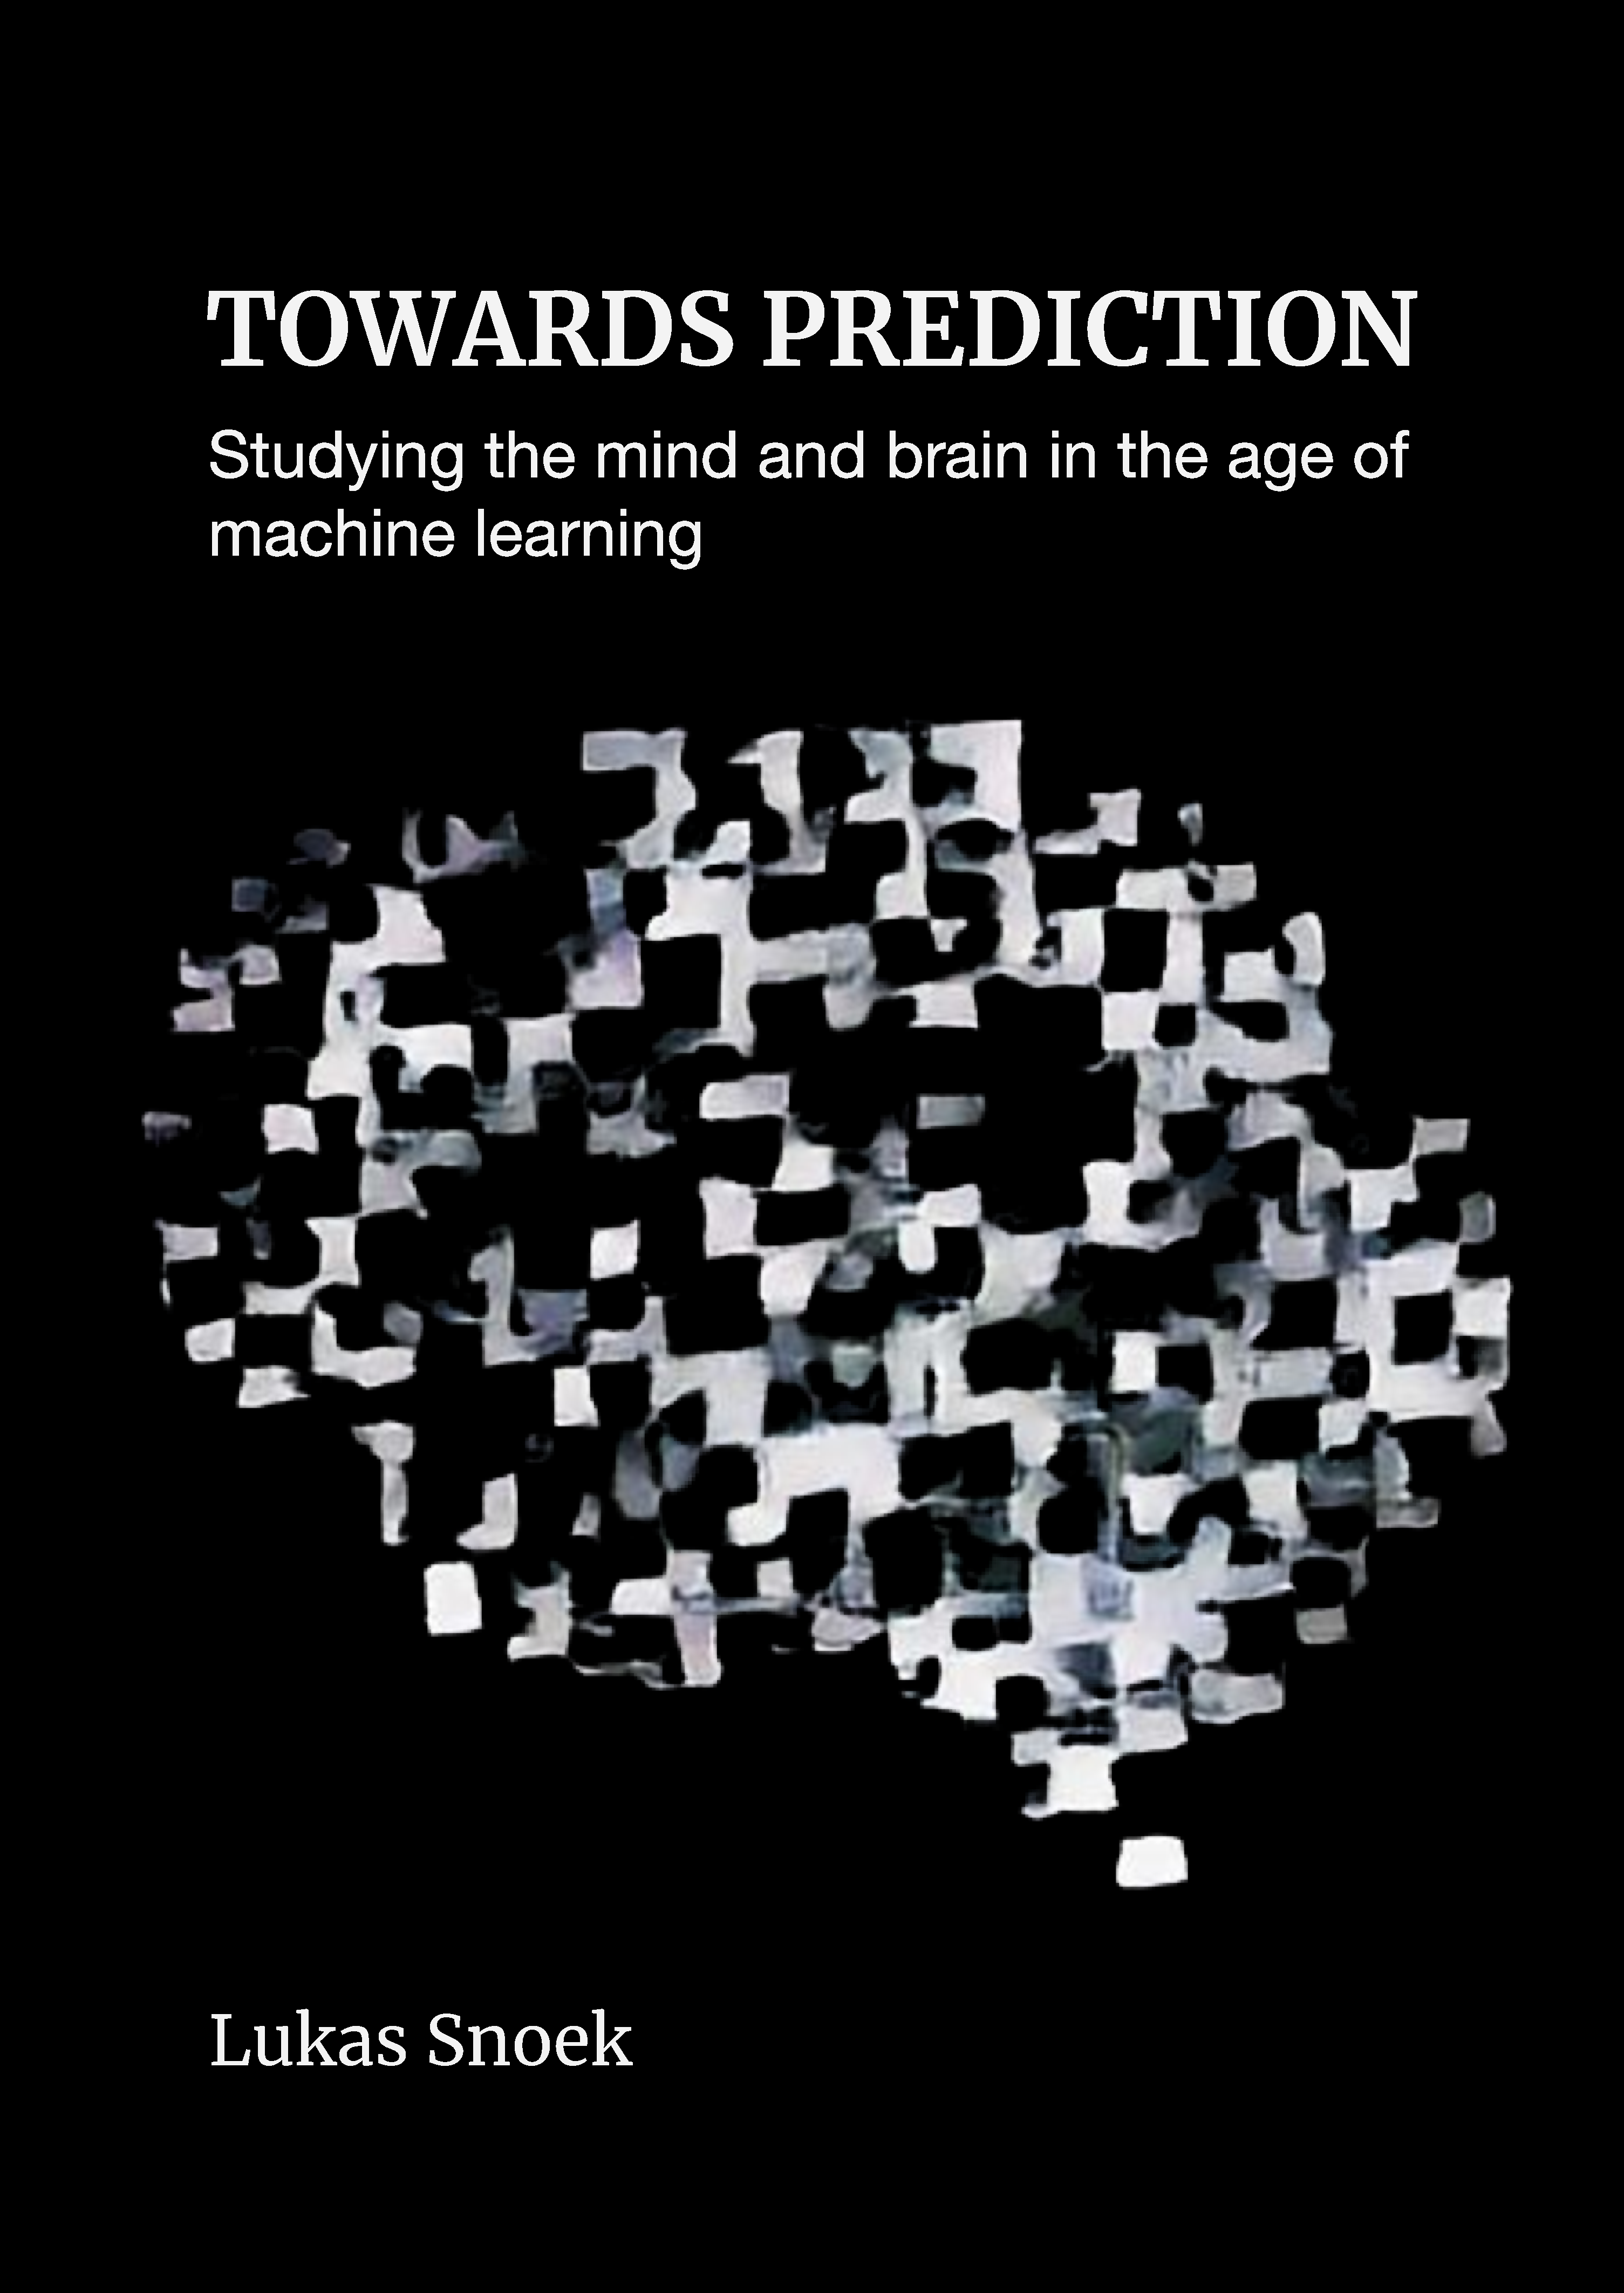
\includepdf{./cover/thesis_cover.pdf}

% \newlength{\mylen}                % a length
% \newcommand{\alphabet}{abcdefghijklmnopqrstuvwxyz} % the lowercase alphabet
% \begingroup                       % keep font change local% font specification e.g., \Large\sffamily
% \settowidth{\mylen}{\alphabet}
% The length of this alphabet is \the\mylen. % print in document\typeout{The length of the Large sans alphabetis \the\mylen}                    % put in log file
% \endgroup                         % end the grouping

{
\setcounter{tocdepth}{1}
\tableofcontents
}
\mainmatter
\hypertarget{introduction}{%
\chapter{Introduction}\label{introduction}}

\emph{The first chapter of the thesis, which introduces your PhD project. The filler-text below was created with the \href{http://www.elsewhere.org/journal/pomo}{postmodernism generator}.}

\begin{center}\rule{0.5\linewidth}{0.5pt}\end{center}

Something about the coming about of this thesis. More of a ``lessons learned'' rather than a coherent research topic.

\hypertarget{the-brain-is-not-a-dictionary}{%
\section{The brain is not a dictionary}\label{the-brain-is-not-a-dictionary}}

Something about looking at populations of neurons/voxels/areas rather than simple one-to-one relationships. Shared states.

\hypertarget{the-brain-probably-does-not-care-about-your-hypothesis}{%
\section{The brain (probably) does not care about your hypothesis}\label{the-brain-probably-does-not-care-about-your-hypothesis}}

Facial expression models.

\hypertarget{interpretability-and-prediction-are-a-trade-off-for-now}{%
\section{Interpretability and prediction are a trade-off (for now)}\label{interpretability-and-prediction-are-a-trade-off-for-now}}

A plea for prediction but a cautionary tale for interpreting predictive models (confounds)

\hypertarget{exploration-should-be-embraced-more}{%
\section{Exploration should be embraced more}\label{exploration-should-be-embraced-more}}

Something about the ``context of discovery'' (cf.~TCM), preregistration, and confirmation vs.~exploration (Morbid curiosity.)

\hypertarget{proper-generalization-is-hard}{%
\section{Proper generalization is hard}\label{proper-generalization-is-hard}}

Within and between subject variance is not noise, but unexplained variance (AU limitations).

\hypertarget{psychology-is-complex-so-it-needs-complex-models}{%
\section{Psychology is complex, so it needs complex models}\label{psychology-is-complex-so-it-needs-complex-models}}

Which need to be fit on complex, large datasets. (AOMIC)

\hypertarget{shared-states}{%
\chapter{Shared states: using MVPA to test neural overlap between self-focused emotion imagery and other-focused emotion understanding}\label{shared-states}}

\chaptermark{Shared states}

\vspace*{\fill}

\begin{center}\rule{0.5\linewidth}{0.5pt}\end{center}

\small

\noindent
\emph{This chapter has been published as}: Oosterwijk, S.*, Snoek, L.*, Rotteveel, M., Barrett, L. F., \& Scholte, H. S. (2017). Shared states: using MVPA to test neural overlap between self-focused emotion imagery and other-focused emotion understanding. \emph{Social cognitive and affective neuroscience, 12}(7), 1025-1035.

* Shared first authorship
\newpage
\normalsize

\textbf{Abstract}

The present study tested whether the neural patterns that support imagining ``performing an action'', ``feeling a bodily sensation'' or ``being in a situation'' are directly involved in understanding \emph{other people's} actions, bodily sensations and situations. Subjects imagined the content of short sentences describing emotional actions, interoceptive sensations and situations (self-focused task), and processed scenes and focused on \emph{how} the target person was expressing an emotion, \emph{what} this person was feeling, and \emph{why} this person was feeling an emotion (other-focused task). Using a linear support vector machine classifier on brain-wide multi-voxel patterns, we accurately decoded each individual class in the self-focused task. When generalizing the classifier from the self-focused task to the other-focused task, we also accurately decoded whether subjects focused on the emotional actions, interoceptive sensations and situations of \emph{others}. These results show that the neural patterns that underlie self-imagined experience are involved in understanding the experience of other people. This supports the theoretical assumption that the basic components of emotion experience and understanding share resources in the brain.

\hypertarget{shared-states-introduction}{%
\section{Introduction}\label{shared-states-introduction}}

To navigate the social world successfully it is crucial to understand other people. But how do people generate meaningful representations of other people's actions, sensations, thoughts and emotions? The dominant view assumes that representations of other people's experiences are supported by the same neural systems as those that are involved in generating experience in the self (e.g., Gallese et al., \protect\hyperlink{ref-gallese2004unifying}{2004}; see for an overview Singer, \protect\hyperlink{ref-singer2012past}{2012}). We tested this principle of self-other neural overlap directly, using multi-voxel pattern analysis (MVPA), across three different aspects of experience that are central to emotions: actions, sensations from the body and situational knowledge.

In recent years, evidence has accumulated that suggests a similarity between the neural patterns representing the self and others. For example, a great variety of studies have shown that observing actions and sensations in other people engages similar neural circuits as acting and feeling in the self (see for an overview Bastiaansen et al., \protect\hyperlink{ref-bastiaansen2009evidence}{2009}). Moreover, an extensive research program on pain has demonstrated an overlap between the experience of physical pain and the observation of pain in other people, utilizing both neuroimaging techniques (e.g., Lamm et al., \protect\hyperlink{ref-lamm2011meta}{2011}) and analgesic interventions (e.g., Rütgen et al., \protect\hyperlink{ref-rutgen2015placebo}{2015}; Mischkowski et al., \protect\hyperlink{ref-mischkowski2016painkiller}{2016}). This process of ``vicarious experience'' or ``simulation'' is viewed as an important component of empathy (Carr et al., \protect\hyperlink{ref-carr2003neural}{2003}; Decety, \protect\hyperlink{ref-decety2011dissecting}{2011}; Keysers \& Gazzola, \protect\hyperlink{ref-keysers2014dissociating}{2014}). In addition, it is argued that mentalizing (e.g.~understanding the mental states of other people) involves the same brain networks as those involved in self-generated thoughts (Uddin et al., \protect\hyperlink{ref-uddin2007self}{2007}; Waytz \& Mitchell, \protect\hyperlink{ref-waytz2011two}{2011}). Specifying this idea further, a constructionist view on emotion proposes that both emotion experience and interpersonal emotion understanding are produced by the same large-scale distributed brain networks that support the processing of sensorimotor, interoceptive and situationally relevant information (Barrett \& Satpute, \protect\hyperlink{ref-barrett2013large}{2013}; Oosterwijk \& Barrett, \protect\hyperlink{ref-oosterwijk2014embodiment}{2014}). An implication of these views is that the representation of self- and other-focused emotional actions, interoceptive sensations and situations overlap in the brain.

Although there is experimental and theoretical support for the idea of self-other neural overlap, the present study is the first to directly test this process using MVPA across three different aspects of experience (i.e.~actions, interoceptive sensations and situational knowledge). Our experimental design consisted of two different tasks aimed at generating self- and other-focused representations with a relatively large weight given to either action information, interoceptive information or situational information.

In the \emph{self-focused} emotion imagery task (SF-task) subjects imagined performing or experiencing actions (e.g., \emph{pushing someone away}), interoceptive sensations (e.g., \emph{increased heart rate}) and situations (e.g., \emph{alone in a park at night}) associated with emotion. Previous research has demonstrated that processing linguistic descriptions of (emotional) actions and feeling states can result in neural patterns of activation associated with, respectively, the representation and generation of actions and internal states (Oosterwijk et al., \protect\hyperlink{ref-oosterwijk2015concepts}{2015}; Pulvermüller \& Fadiga, \protect\hyperlink{ref-pulvermuller2010active}{2010}). Furthermore, imagery-based inductions of emotion have been successfully used in the MRI scanner before (Oosterwijk et al., \protect\hyperlink{ref-oosterwijk2012states}{2012}; Wilson-Mendenhall et al., \protect\hyperlink{ref-wilson2011grounding}{2011}), and are seen as robust inducers of emotional experience (Lench et al., \protect\hyperlink{ref-lench2011discrete}{2011}). In the \emph{other-focused} emotion understanding task (OF-task), subjects viewed images of people in emotional situations and focused on actions (i.e., \emph{How} does this person express his/her emotions?), interoceptive sensations (i.e., \emph{What} does this person feel in his/her body) or the situation (i.e., \emph{Why} does this person feel an emotion?). This task is based on previous research studying the neural basis of emotion oriented mentalizing (Spunt \& Lieberman, \protect\hyperlink{ref-spunt2012integrative}{2012}).

With MVPA, we examined to what extent the SF- and OF-task evoked similar neural patterns. MVPA allows researchers to assess whether the neural pattern associated with one set of experimental conditions can be used to distinguish between another set of experimental conditions. This relatively novel technique has been successfully applied to the field of social neuroscience in general (e.g., Gilbert et al., \protect\hyperlink{ref-gilbert2012evaluative}{2012}; Brosch et al., \protect\hyperlink{ref-brosch2013implicit}{2013}; Parkinson et al., \protect\hyperlink{ref-parkinson2014common}{2014}), and the field of self-other neural overlap in particular. For example, several MVPA studies recently assessed whether experiencing pain and observing pain in others involved similar neural patterns (Corradi-Dell'Acqua et al., \protect\hyperlink{ref-corradi2016cross}{2016}; Krishnan et al., \protect\hyperlink{ref-krishnan2016somatic}{2016}). Although there is an ongoing discussion about the specifics of shared representation in pain based on these MVPA results (see for an overview Zaki et al., \protect\hyperlink{ref-zaki2016anatomy}{2016}), many authors emphasize the importance of this technique in the scientific study of self-other neural overlap (e.g., Corradi-Dell'Acqua et al., \protect\hyperlink{ref-corradi2016cross}{2016}; Krishnan et al., \protect\hyperlink{ref-krishnan2016somatic}{2016}).

MVPA is an analysis technique that decodes latent categories from fMRI data in terms of multi-voxel patterns of activity (Norman et al., \protect\hyperlink{ref-norman2006beyond}{2006}\protect\hyperlink{ref-norman2006beyond}{a}). This technique is particularly suited for our research question for several reasons. First of all, although univariate techniques can demonstrate that tasks activate the same brain regions, only MVPA can statistically test for shared representation (Lamm \& Majdandžić, \protect\hyperlink{ref-lamm2015role}{2015}). We will evaluate whether multivariate brain patterns that distinguish between mental events in the SF-task can be used to distinguish, above chance level, between mental events in the OF-task. Second, MVPA analyses are particularly useful in research that is aimed at examining distributed representations (Singer, \protect\hyperlink{ref-singer2012past}{2012}). Based on our constructionist framework, we indeed hypothesize that the neural patterns that will represent self- and other focused mental events are distributed across large-scale brain networks. To capture these distributed patterns, we used MVPA in combination with data-driven univariate feature selection on whole-brain voxel patterns, instead of limiting our analysis to specific regions-of-interest (Haynes, \protect\hyperlink{ref-haynes2015primer}{2015}). And third, in contrast to univariate analyses that aggregate data across subjects, MVPA can be performed within-subjects and is thus able to incorporate individual variation in the representational content of multivariate brain patterns. In that aspect within-subject MVPA is sensitive to individual differences in how people imagine actions, sensations and situations, and how they understand others. In short, for our purpose to explicitly test the assumption that self and other focused processes share neural resources, MVPA is the designated method.

We tested the following two hypotheses. First, we tested whether we could classify \emph{self-imagined} actions, interoceptive sensations and situations above chance level. Second, we tested whether the multivariate pattern underlying this classification could also be used to classify the how, what and why condition in the \emph{other-focused} task.

\hypertarget{shared-states-methods}{%
\section{Methods}\label{shared-states-methods}}

\hypertarget{shared-states-methods-subjects}{%
\subsection{Subjects}\label{shared-states-methods-subjects}}

In total, we tested 22 Dutch undergraduate students from the University of Amsterdam (14 females; M\textsubscript{age} = 21.48, s.d.\textsubscript{age} = 1.75). Of those 22 subjects, 13 subjects were tested twice in 2 sessions about 1 week apart. Half of those sessions were used for the model optimization procedure. The other half of the sessions, combined with an additional nine subjects (who were tested only once), constituted the model validation set (see Model optimization procedure section). In total, two subjects were excluded from the model validation dataset: one subject was excluded because there was not enough time to complete the experimental protocol and another subject was excluded due to excessive movement (\textgreater3 mm within data acquisition runs).

All subjects signed informed consent prior to the experiment. The experiment was approved by the University of Amsterdam's ethical review board. Subjects received 22.50 euro per session. Standard exclusion criteria regarding MRI safety were applied and people who were on psychopharmacological medication were excluded a priori.

\hypertarget{shared-states-methods-experimental-design}{%
\subsection{Experimental design}\label{shared-states-methods-experimental-design}}

\hypertarget{shared-states-methods-experimental-design-sf-task}{%
\subsubsection{Self-focused emotion imagery task}\label{shared-states-methods-experimental-design-sf-task}}

The self-focused emotion imagery task (SF-task) was created to preferentially elicit \emph{self-focused} processing of action, interoceptive or situational information associated with emotion. Subjects processed short linguistic cues that described actions (e.g., \emph{pushing someone away}; \emph{making a fist}), interoceptive sensations (e.g., \emph{being out of breath}; \emph{an increased heart rate}), or situations (e.g., \emph{alone in a park at night}; \emph{being falsely accused}) and were instructed to imagine performing or experiencing the content. The complete instruction is presented in the Supplementary Materials; all stimuli used in the SF-task are presented in Supplementary Table \ref{tab:tab-shared-states-S1}. Linguistic cues were selected from a pilot study performed on an independent sample of subjects (\emph{n} = 24). Details about this pilot study are available on request. The descriptions generated in this pilot study were used as qualitative input to create short sentences that described actions, sensations or situations that were associated with negative emotions, without including discrete emotion terms. The cues did not differ in number of words, nor in number of characters (\emph{F} \textless{} 1).

The SF-task was performed in two runs subsequent to the other-focused task using the software package Presentation (Version 16.4, \url{www.neurobs.com}). Each run presented 60 sentences on a black background (20 per condition) in a fully randomized event-related fashion, with a different randomization for each subject. Note that implementing a separate randomization for each subject prevents inflated false positive pattern correlations between trials of the same condition, which may occur in single-trial designs with short inter-stimulus intervals (Mumford et al., \protect\hyperlink{ref-mumford2014impact}{2014}). A fixed inter-trial--interval of 2 seconds separating trials; 12 null-trials (i.e.~a black screen for 8 seconds) were mixed with the experimental trials at random positions during each run (see Figure \ref{fig:fig-shared-states-1}).

\begin{figure}
\centering
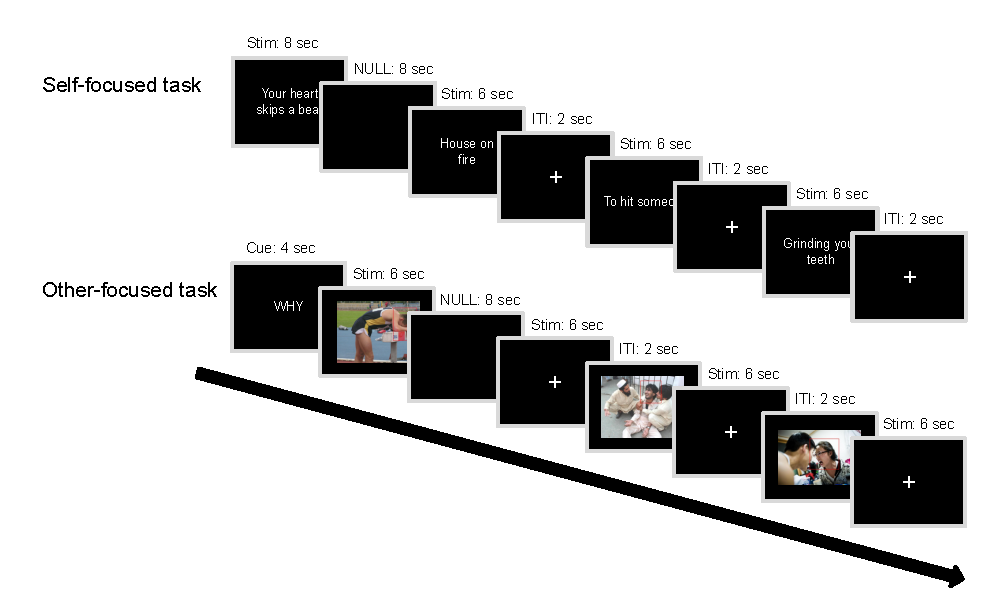
\includegraphics{_bookdown_files/shared-states-files/figures/figure_1.pdf}
\caption{\label{fig:fig-shared-states-1}Overview of the self-focused and other-focused task.}
\end{figure}

\hypertarget{shared-states-methods-experimental-design-of-task}{%
\subsubsection{Other-focused emotion understanding task}\label{shared-states-methods-experimental-design-of-task}}

The other-focused emotion understanding task (OF-task) was created to preferentially elicit \emph{other-focused} processing of action, interoceptive or situational information associated with emotion. Subjects viewed images of people in negative situations (e.g.~a woman screaming at a man, a man held at gunpoint). A red rectangle highlighted the face of the person that the subjects should focus on to avoid ambiguity in images depicting more than one person. Image blocks were preceded by a cue indicating the strategy subjects should use in perceiving the emotional state of the people in the images (Spunt \& Lieberman, \protect\hyperlink{ref-spunt2012integrative}{2012}). The cue \emph{How} instructed the subjects to identify actions that were informative about the person's emotional state (i.e., \emph{How} does this person express his/her emotions?). The cue \emph{What} instructed subjects to identify interoceptive sensations that the person could experience (i.e., \emph{What} does this person feel in his/her body). The cue \emph{Why} instructed subjects to identify reasons or explanations for the person's emotional state (i.e., \emph{Why} does this person feel an emotion?). The complete instruction is presented in the \protect\hyperlink{shared-states-supplement}{Supplementary Materials}.

Stimuli for the OF-task were selected from the International Affective Picture System database (IAPS; Lang, \protect\hyperlink{ref-lang2005international}{2005}; Lang et al., \protect\hyperlink{ref-lang1997international}{1997}), the image set developed by the Kveraga lab (\url{http://www.kveragalab.org/stimuli.html}; Kveraga et al., \protect\hyperlink{ref-kveraga2015if}{2015}) and the internet (Google images). We selected images based on a pilot study, performed on an independent sample of subjects (\emph{n} = 22). Details about this pilot study are available on request.

The OF-task was presented using the software package Presentation. The task presented thirty images on a black background in blocked fashion, with each block starting with a what, why or how cue (see Figure \ref{fig:fig-shared-states-1}). Each image was shown three times, once for each cue type. Images were presented in blocks of six, each lasting 6 seconds, followed by a fixed inter trial interval of 2 seconds. Null-trials were inserted at random positions within the blocks. Both the order of the blocks and the specific stimuli within and across blocks were fully randomized, with a different randomization for each subject.

\hypertarget{shared-states-methods-procedure}{%
\subsection{Procedure}\label{shared-states-methods-procedure}}

Each experimental session lasted about 2 hours. Subjects who underwent two sessions had them on different days within a time span of 1 week. On arrival, subjects gave informed consent and received thorough task instructions, including practice trials (see the \protect\hyperlink{shared-states-supplement}{Supplementary Materials} for a translation of the task instructions). The actual time in the scanner was 55 minutes, and included a rough 3D scout image, shimming sequence, 3-min structural T1-weighted scan, one functional run for the OF-task and two functional runs for the SF-task. We deliberately chose to present the SF-task after the OF-task to exclude the possibility that the SF-task affected the OF-task, thereby influencing the success of the decoding procedure.

After each scanning session, subjects rated their success rate for the SF-task and OF-task (see Supplementary Figure \ref{fig:fig-shared-states-S1}). In the second session, subjects filled out three personality questionnaires that will not be further discussed in this paper and were debriefed about the purpose of the study.

\hypertarget{shared-states-methods-image-acquisition}{%
\subsection{Image acquisition}\label{shared-states-methods-image-acquisition}}

Subjects were tested using a Philips Achieva 3T MRI scanner and a 32-channel SENSE headcoil. A survey scan was made for spatial planning of the subsequent scans. Following the survey scan, a 3-min structural T1-weighted scan was acquired using 3D fast field echo (TR: 82 ms, TE: 38 ms, flip angle: 8°, FOV: 240 × 188 mm, 220 slices acquired using single-shot ascending slice order and a voxel size of 1.0 × 1.0 × 1.0 mm). After the T1-weighted scan, functional T2*-weighted sequences were acquired using single shot gradient echo, echo planar imaging (TR = 2000 ms, TE = 27.63 ms, flip angle: 76.1°, FOV: 240 × 240 mm, in-plane resolution 64 × 64, 37 slices (with ascending acquisition), slice thickness 3 mm, slice gap 0.3 mm, voxel size 3 × 3 × 3 mm), covering the entire brain. For the SF-task, 301 volumes were acquired; for the OF-task 523 volumes were acquired.

\hypertarget{shared-states-methods-model-optimization-procedure}{%
\section{Model optimization procedure}\label{shared-states-methods-model-optimization-procedure}}

As MVPA is a fairly novel technique, no consistent, optimal MVPA pipeline has been established (Etzel et al., \protect\hyperlink{ref-etzel2011impact}{2011}). Therefore, we adopted a validation strategy in the present study that is advised in the pattern classification field (Kay et al., \protect\hyperlink{ref-kay2008identifying}{2008}; Kriegeskorte et al., \protect\hyperlink{ref-kriegeskorte2009circular}{2009}). This strategy entailed that we separated our data into an optimization dataset to find the most optimal parameters for preprocessing and analysis, and a validation dataset to independently verify classification success with those optimal parameters. We generated an optimization and validation dataset by running the SF-task and OF-task twice, in two identical experimental sessions for a set of thirteen subjects. The sessions were equally split between the optimization and validation set (see Figure 2A); first and second sessions were counterbalanced between the two sets. Based on a request received during the review process, we added nine new subjects to the validation dataset. Ultimately, the optimization-set held 13 sessions and the validation-set, after exclusion of 2 subjects (see Subjects section), held 20 sessions.

\begin{figure}
\centering
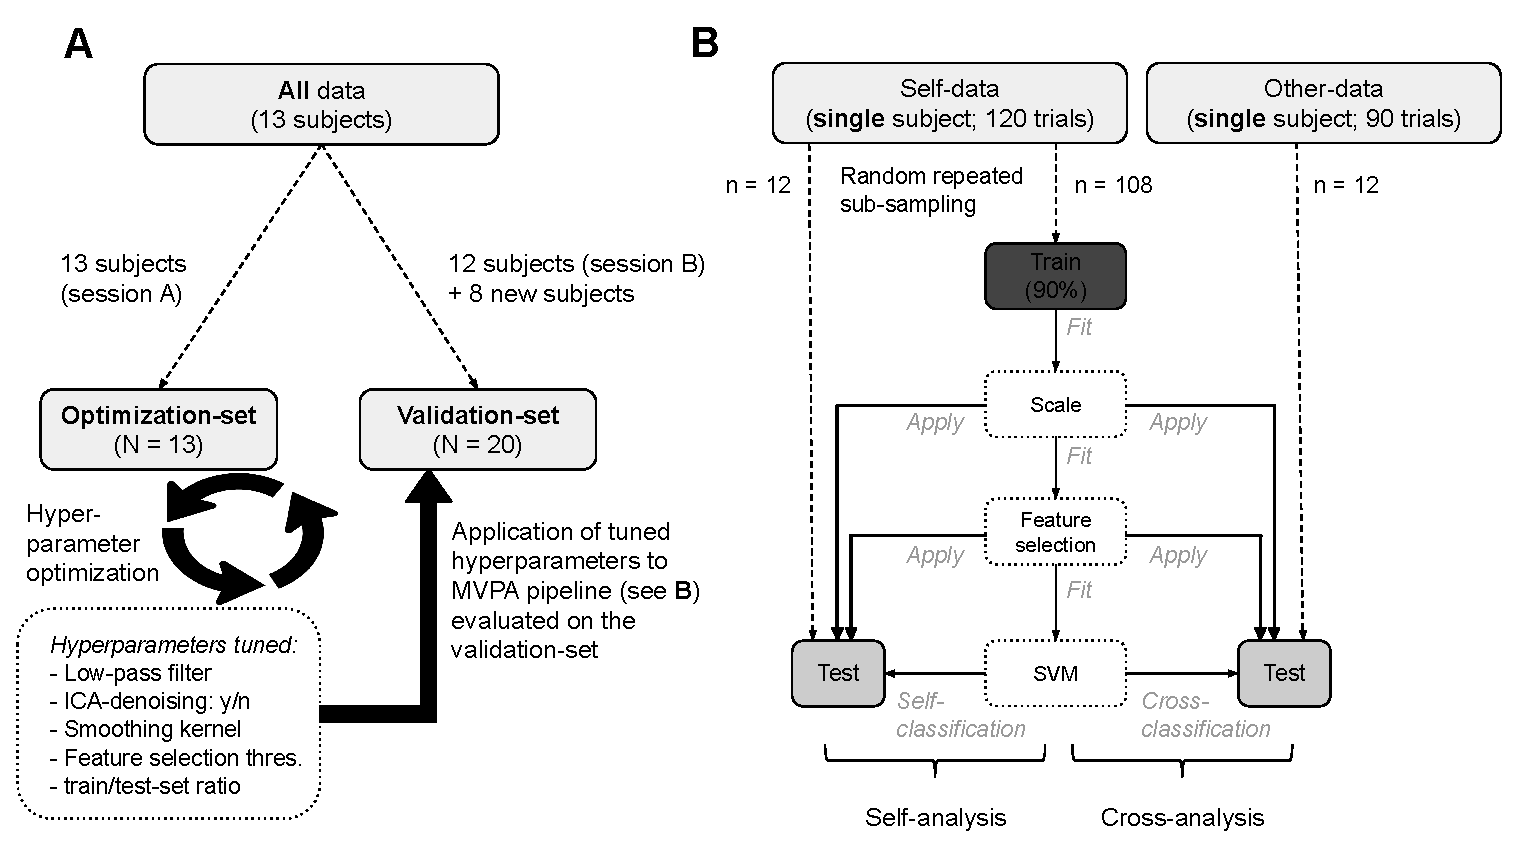
\includegraphics{_bookdown_files/shared-states-files/figures/figure_2.pdf}
\caption{\label{fig:fig-shared-states-2}Schematic overview of the cross-validation procedures. \textbf{A}) The partitioning of the dataset into an optimization-set (used for tuning of preprocessing and MVPA hyperparameters) and a validation-set (used to get a fully cross-validated, unbiased estimate of classification performance). The preprocessing and MVPA hyperparameters yielded from the optimization procedure were subsequently applied to the preprocessing and MVPA pipeline of the validation-set. \textbf{B}) The within-subject MVPA pipeline of the self- and cross-analysis implemented in a repeated random subsampling scheme with 100,000 iterations. In each iteration, 90\% of the self-data trials (i.e.~train-set) were used for estimating the scaling parameters, performing feature selection and fitting the SVM. These steps of the pipeline (i.e.~scaling, feature selection, SVM fitting) were subsequently applied to the independent test-set of both the self-data trials and the other-data trials.}
\end{figure}



In the optimization-set, we explored how different preprocessing options and the so-called `hyperparameters' in the MVPA pipeline affected the performance of the (multivariate) analyses (visualized in Figure \ref{fig:fig-shared-states-2}B; see \protect\hyperlink{shared-states-methods-mvpa-pipeline}{MVPA pipeline} subsection for more details). Thus, we performed the self- and cross-analyses \emph{on the data of the optimization set} multiple times with different preprocessing options (i.e., smoothing kernel, low-pass filter and ICA-based denoising strategies) and MVPA hyperparameter values (i.e., univariate feature selection \emph{threshold} and train/test size ratio during cross-validation). We determined the optimal parameters on the basis of classification performance, which was operationalized as the mean precision value after a repeated random subsampling procedure with 1000 iterations. A list with the results from the optimization procedure can be found in Supplementary Table \ref{tab:tab-shared-states-S2} and Supplementary Figure \ref{fig:fig-shared-states-S2}. The optimal parameters were then used for preprocessing and the self- and cross-analysis within the validation-set, in which the findings from the optimization-set were replicated. All findings discussed in the \ref{shared-states-results} section follow from the validation-set (see Supplementary Figure \ref{fig:fig-shared-states-S3} for an overview of the findings from the optimization-set).

\hypertarget{shared-states-methods-preprocessing}{%
\subsection{Preprocessing and single-trial modeling}\label{shared-states-methods-preprocessing}}

Functional and structural data were preprocessed and analyzed using FSL 5.0 (Jenkinson et al., \protect\hyperlink{ref-jenkinson2012fsl}{2012}) and MATLAB (2012b; \url{www.mathworks.com/products/matlab}), using an in-house developed preprocessing pipeline and the parameters established in the optimization procedure. Functional data were corrected for motion (using FSL MCFLIRT) and slice timing and was spatially smoothed (5 mm isotropic kernel). After preprocessing, individual time series were modeled using a double-gamma hemodynamic response function in a single-trial GLM design using FSL's FEAT. Resulting beta values were converted to \emph{t}-values (Misaki et al., \protect\hyperlink{ref-misaki2010comparison}{2010}), constituting a whole-brain pattern of \emph{t}-values per trial. Subsequently, the data were indexed by a gray-matter mask (excluding most white-matter, CSF and brainstem voxels). Thus, the data points for the MVPA consist of whole-brain (gray matter) \emph{t}-value patterns per trial. For the optimization analyses, the data were transformed to standard space (MNI152, 2 mm) using FSL's FNIRT. To reduce computation time for the validation data, and in particular its corresponding permutation analysis, analyses on the validation dataset were performed on data in native (functional) space.

\hypertarget{shared-states-methods-mvpa}{%
\subsection{Multi-voxel pattern analysis}\label{shared-states-methods-mvpa}}

\hypertarget{shared-states-methods-mvpa-pipeline}{%
\subsubsection{MVPA pipeline}\label{shared-states-methods-mvpa-pipeline}}

Within the optimization and validation dataset, we implemented an iterated cross-validation scheme that separated the data into a train-set and a test-set (this procedure is described in more detail in the next section). Before fitting the classifier on the train-set in each iteration of the cross-validation scheme, standardization and voxel selection were estimated and applied to the train-set. Standardization ensured that each feature (i.e., voxel) had zero mean and unit variance across trials. After standardization, voxel selection was performed in each iteration on the train-set by extracting the voxels with the highest average pairwise Euclidian distance across classes, which will be subsequently referred to as a voxel's differentiation score. More specifically, differentiation scores were calculated by subtracting the mean value across trials per class from each other (i.e., action---interoception, action---situation, interoception---situation), normalizing these values across voxels (yielding ``z-scores''), and taking their absolute value. The three resulting values per voxel were averaged and the most differentiating voxels (z-score threshold: 2.3, as determined by the optimization procedure; see \protect\hyperlink{shared-states-methods-model-optimization-procedure}{Model optimization procedure} section) were extracted and used as features when fitting the classifier. Importantly, the standardization parameters (voxel mean and variance) and voxel indices (i.e.~which voxels had differentiation scores above threshold) were estimated from the train-set only and subsequently applied to the test-set to ensure independence between the train- and test-set (see Figure 2B). After standardization and voxel selection in each iteration, a support vector classifier (SVC) was fit on the train-set and cross-validated on the test-set, generating a class probability for each trial in the test-set. Our classifier of choice was the SVC implementation from the scikit-learn \texttt{svm} module (Pedregosa et al., \protect\hyperlink{ref-pedregosa2011scikit}{2011}) with a linear kernel, fixed regularization parameter (\emph{C}) of 1.0, one-vs-one multiclass strategy, estimation of class probability output (instead of discrete class prediction) and otherwise default parameters.

\hypertarget{shared-states-methods-mvpa-cv-and-bagging}{%
\subsubsection{Cross-validation scheme and bagging procedure}\label{shared-states-methods-mvpa-cv-and-bagging}}

Cross-validation of the classification analysis was implemented using a repeated random subsampling cross-validation scheme (also known as Monte Carlo cross-validation), meaning that, for each iteration of the analysis, the classification pipeline (i.e., standardization, voxel selection and SVM fitting) was applied on a random subset of data points (i.e., the train-set) and cross-validated on the remaining data (i.e., the test-set). Each trial belonged to one out of three classes: action, interoception or situation. Following the results from the parameter optimization process, we selected four trials per class for testing, amounting to 12 test-trials per iteration.

Per iteration, the classifier was fit on the train-set from the SF-data. Subsequently, this classifier was cross-validated on 12 test SF-trials (test-set ``self-analysis'') and 12 test OF-trials (test-set ``cross-analysis''; see Figure 2B). This process was subsequently iterated 100 000 times to generate a set of class distributions for each trial. After all iterations, the final predicted class of each trial was determined by its highest summed class probability across iterations (also known as ``soft voting''; see Supplementary Figure \ref{fig:fig-shared-states-S4}). This strategy of a random sub-sampling cross-validation scheme in combination with majority (soft) voting is more commonly known as ``bagging'' (Breiman, \protect\hyperlink{ref-breiman1996bagging}{1996}). An important advantage of bagging is that it reduces model overfitting by averaging over an ensemble of models, which is especially useful for multi-voxel pattern analyses because fMRI data is known to display high variance (Varoquaux, \protect\hyperlink{ref-varoquaux2018cross}{2018}).

After generating a final prediction for all trials using the soft voting method, we constructed confusion matrices for both the self- and cross-analysis. In each raw confusion matrix with prediction counts per class, cells were normalized by dividing prediction counts by the sum over rows (i.e., the total amount of predictions per class), yielding precision-scores (also known as positive predictive value). In other words, this metric represents the ratio of true positives to the sum of true positives and false positives (see Supplementary Figure \ref{fig:fig-shared-states-S5} for a description of the results expressed as \emph{recall} estimates, or the ratio of true positives to the total number of samples in that class). This classification pipeline generated subject-specific confusion matrices that were subsequently averaged to generate the final classification scores.

\hypertarget{shared-states-methods-mvpa-statistical-evaluation}{%
\subsubsection{Statistical evaluation}\label{shared-states-methods-mvpa-statistical-evaluation}}

To evaluate the statistical significance of the observed average precision-scores in the confusion matrices, we permuted the original self- and cross-analysis 1300 times per subject with randomly shuffled class labels, yielding 1300 confusion matrices (with precision-scores). We then averaged the confusion matrices across subjects, yielding 1300 permuted confusion matrices reflecting the null-distribution of each cell of the matrix (which is centered around chance level classification, i.e., 33\%). For each cell in the diagonal of the observed confusion matrix, \emph{p}-values were calculated as the proportion of instances of values in the permuted matrix which were higher than the values in the observed matrix (Nichols \& Holmes, \protect\hyperlink{ref-nichols2002nonparametric}{2002}). To correct for multiple comparisons, \emph{p}-values were tested against a Bonferroni-corrected threshold. The distribution of precision-scores and the relationship between precision-scores in the self- and cross-analysis is reported in Supplementary Figure \ref{fig:fig-shared-states-S6}.

\hypertarget{shared-states-methods-mvpa-spatial-representation}{%
\subsubsection{Spatial representation}\label{shared-states-methods-mvpa-spatial-representation}}

To visualize the classifier feature weights, we plotted the absolute feature weights averaged over iterations, subjects and pairwise classifiers (action \emph{vs} interoception, action \emph{vs} situation, interoception \emph{vs} situation) that underlie our multiclass classification analysis. We chose to visualize the spatial representation of our model by plotting the average absolute feature weights, because the absolute value of feature weights in linear SVMs can be interpreted as how important the weights are in constructing the model's decision hyperplane (Ethofer et al., \protect\hyperlink{ref-ethofer2009decoding}{2009}; Guyon et al., \protect\hyperlink{ref-guyon2002gene}{2002}; Stelzer et al., \protect\hyperlink{ref-stelzer2014prioritizing}{2014}). To correct for a positive bias in plotting absolute weights, we ran the main classification analysis again with permuted labels to extract the average absolute feature weights that one would expect by chance. Subsequently, a voxel-wise independent \emph{t}-test was performed for all feature weights across subjects, using the average permuted feature weights as the null-hypothesis, yielding an interpretable \emph{t}-value map (see the supplementary code notebook on our Github repository for computational details).

\hypertarget{shared-states-methods-additional-analyses}{%
\subsection{Additional analyses}\label{shared-states-methods-additional-analyses}}

In addition to the self-analysis and the self-to-other cross-analysis presented in the main text, we also performed a within-subjects other-to-self cross-analysis (see for a similar approach Corradi-Dell'Acqua et al., \protect\hyperlink{ref-corradi2016cross}{2016}) and a between-subjects self-analysis and self-to-other cross-analysis. These analyses forward largely similar results as the analyses presented in the main text. Due to space constraints, we present these additional analyses in the \protect\hyperlink{shared-states-supplement}{Supplementary Materials}. Supplementary Figure \ref{fig:fig-shared-states-S7} represents confusion matrices with precision and recall estimates for the other-to-self cross-analysis. Supplementary Figure \ref{fig:fig-shared-states-S8} presents the results of MVPA analyses using condition-average voxel patterns across subjects instead of single-trial patterns within subjects.

\hypertarget{shared-states-methods-univariate-analysis}{%
\subsection{Univariate analysis}\label{shared-states-methods-univariate-analysis}}

To be complete, we also report a set of univariate analyses performed on the SF-task and the OF-task data. The univariate analyses were performed on the validation dataset, and were subject to the same preprocessing steps as the MVPA analysis, except that we did not model each trial, but each condition as a separate regressor. The group-level analysis was performed with FSL's FLAME1 option. To examine differences in neural activity between conditions, we calculated contrasts between the three classes in the SF-task (self-action \emph{vs} self-interoception; self-action \emph{vs} self-situation and self-interoception \emph{vs} self-situation) and the three classes in the OF-task (other-action \emph{vs} other-interoception; other-action \emph{vs} other-situation and other-interoception \emph{vs} other-situation). We report clusters that were corrected using cluster-correction with a voxel-wise threshold of 0.005 (\emph{z} = 2.7) and a cluster-wise \emph{p}-value threshold of 0.05.

\hypertarget{shared-states-methods-code-availability}{%
\subsection{Code availability}\label{shared-states-methods-code-availability}}

The MVPA-analysis and subsequent (statistical) analyses were implemented using custom Python scripts, which depend heavily on the skbold package, a set of tools for machine learning analyses of fMRI data developed in-house (see \url{https://github.com/lukassnoek/skbold}). The original scripts were documented and are hosted at the following Github repository: \url{https://github.com/lukassnoek/SharedStates}.

\hypertarget{shared-states-results}{%
\section{Results}\label{shared-states-results}}

\hypertarget{shared-states-results-mvpa}{%
\subsection{Multi-voxel pattern analysis}\label{shared-states-results-mvpa}}

The analyses of the SF-task demonstrated that voxel patterns reflecting imagined self-focused actions, interoceptive sensations and situations associated with emotion could be decoded accurately for each individual class (all \emph{p} \textless{} 0.001, see Figure \ref{fig:fig-shared-states-3}). Furthermore, when we generalized the classifier based on the SF-task to the data from the OF-task (i.e.~cross-analysis), we found that neural representations of emotional actions, interoceptive sensations and situations of others could also be reliably decoded above chance (all \emph{p} \textless{} 0.001; see Figure \ref{fig:fig-shared-states-3}). Supplementary Table \ref{tab:tab-shared-states-S3} presents mean precision-scores across classes for each subject separately. As predicted, our findings demonstrate that \emph{self-imagined} actions, interoceptive sensations and situations are associated with distinct neural patterns. Furthermore, and as predicted, our findings demonstrate that the patterns associated with self-imagined actions, sensations and situations can be used to decode \emph{other-focused} actions, interoceptive sensations and situations (see Supplementary Figure \ref{fig:fig-shared-states-S7} for the complementary other-to-self cross-analysis).

\begin{figure}
\centering
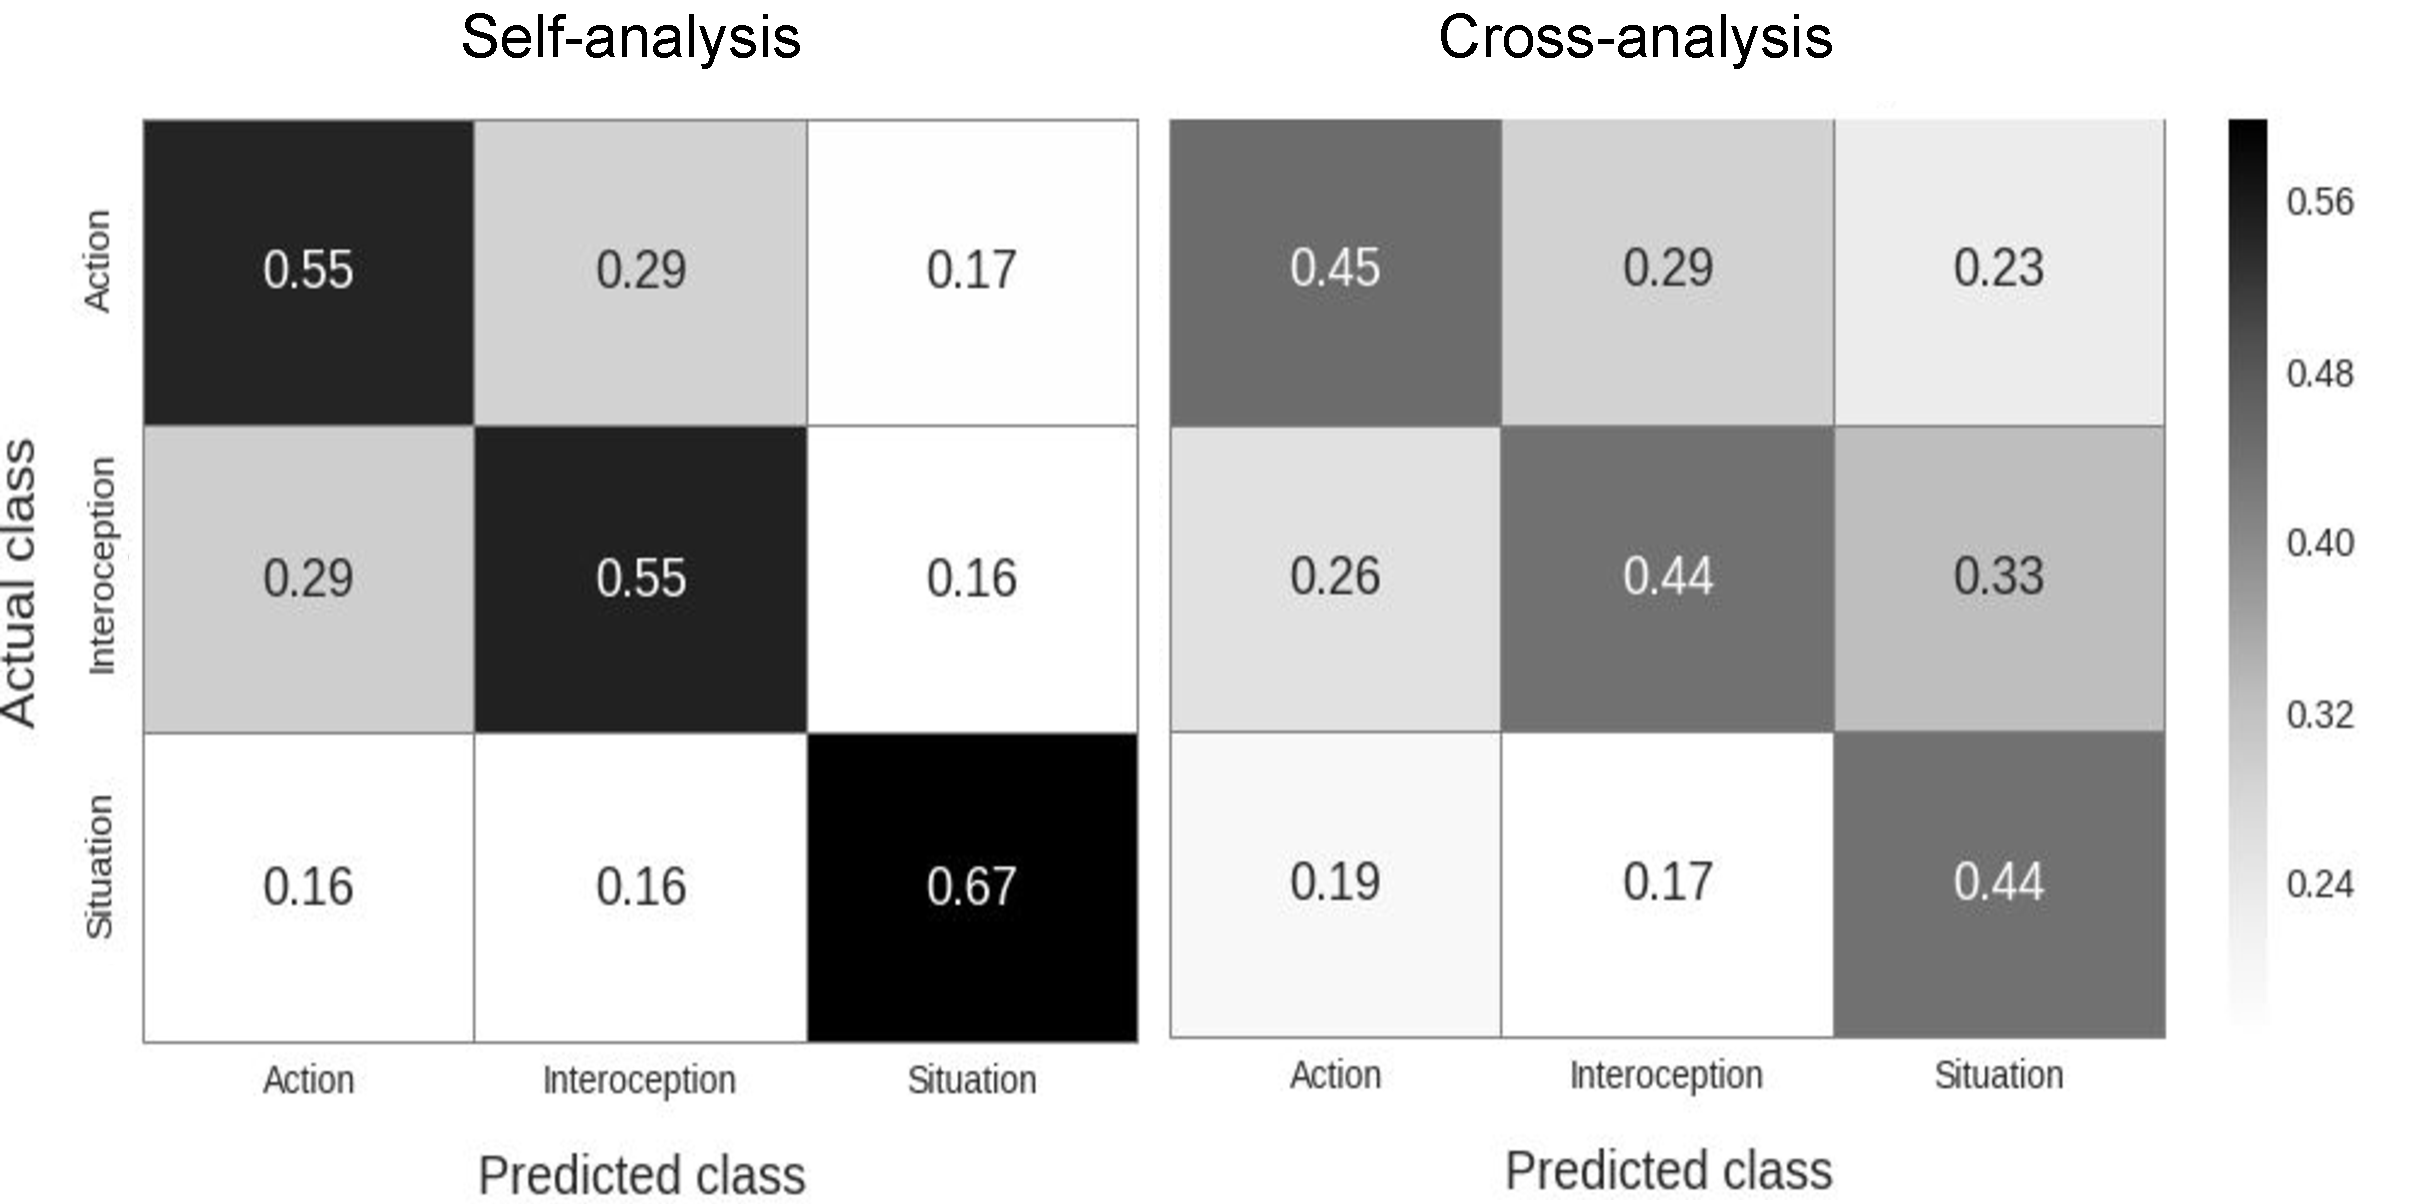
\includegraphics{_bookdown_files/shared-states-files/figures/figure_3.pdf}
\caption{\label{fig:fig-shared-states-3}Confusion matrices for the self- (left diagram) and cross-analysis (right diagram). Values indicate precision-scores, representing the proportion of true positives given all predictions for a certain class. Note that action and interoception columns in the cross-analysis confusion matrix do not add up to 1, which is caused by the fact that, for some subjects, no trials were predicted as action or interoception, rendering the calculation of precision ill-defined (i.e., division by zero). In this case, precision scores were set to zero.}
\end{figure}



To visualize which neural regions were involved in the successful decoding of the three classes in the OF-task and SF-task, we display in Figure \ref{fig:fig-shared-states-4} the averaged absolute values of the SVM feature weights. Note that Figure \ref{fig:fig-shared-states-4} only displays one feature map, as both the self and cross-analysis depend on the same model. Regions displaying high and consistent feature weights across subjects were frontal pole (including parts of the dorsomedial prefrontal cortex and ventromedial prefrontal cortex), orbitofrontal cortex (OFC), inferior frontal gyrus (IFG), superior frontal gyrus (SFG), middle frontal gyrus (MFG), insular cortex, precentral gyrus, postcentral gyrus, posterior cingulate cortex/precuneus, superior parietal lobule (SPL), supramarginal gyrus (SMG), angular gyrus (AG), middle temporal gyrus (MTG), temporal pole (TP), lateral occipital cortex (lOC) and occipital pole (see Supplementary Table \ref{tab:tab-shared-states-S4} for an overview of all involved regions).

\begin{figure}
\centering
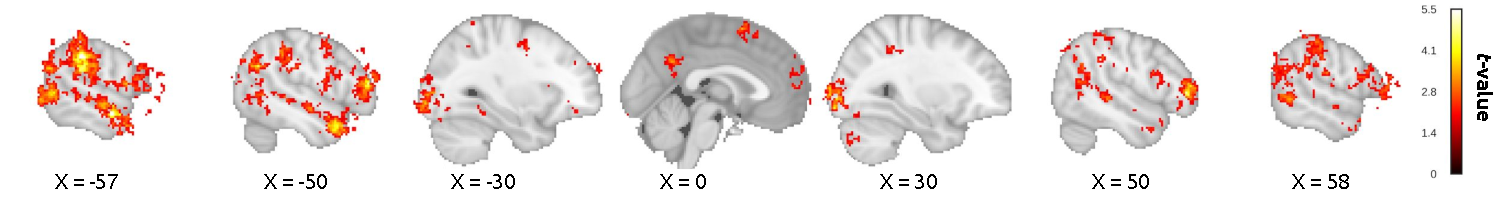
\includegraphics{_bookdown_files/shared-states-files/figures/figure_4.pdf}
\caption{\label{fig:fig-shared-states-4}Uncorrected \emph{t}-value map of average feature weights across subjects; \emph{t}-values were calculated by dividing the average absolute feature weights, which was corrected for positive bias by subtracting the mean permuted absolute weight across all iterations, by the standard error across subjects. Only voxels belonging to clusters of 20 or more voxels are shown.}
\end{figure}



\hypertarget{shared-states-results-univariate}{%
\subsection{Univariate analyses}\label{shared-states-results-univariate}}

Figure \ref{fig:fig-shared-states-5} displays the pattern of neural activity revealed by univariate contrasts between the three different classes in the SF-task and the OF-task. For the sake of brevity, we summarize the most relevant univariate results here. Please see the \protect\hyperlink{shared-states-supplement}{Supplementary Materials} and the study's Github repository for an overview of all clusters.

\begin{figure}
\centering
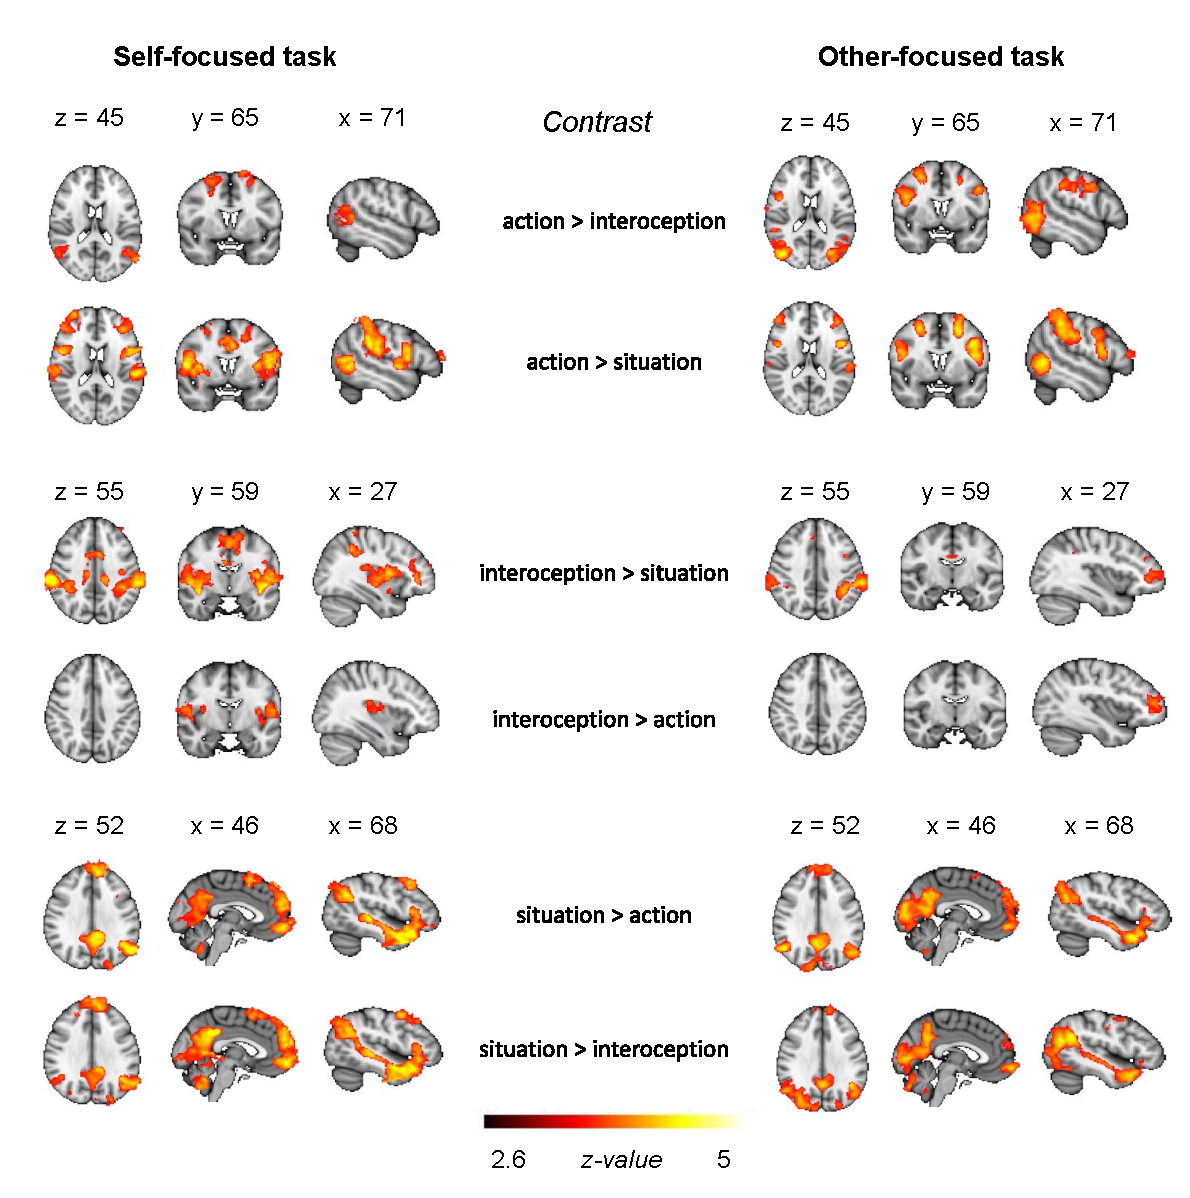
\includegraphics{_bookdown_files/shared-states-files/figures/figure_5.pdf}
\caption{\label{fig:fig-shared-states-5}Univariate contrasts for the self-focused and other-focused task.}
\end{figure}

In the SF-task, action was associated with increased involvement of the MFG, SFG, AG, SMG, lOC and middle temporal gyrus (temporo-occipital) when compared with interoception, and increased involvement of the IFG, MFG, SFG, anterior cingulate cortex (ACC), supplementary motor area (SMA), precentral gyrus, postcentral gyrus, insular cortex, SMG, SPL, lOC and middle temporal gyrus (temporo-occipital) when compared with situation. Interoception was associated with increased involvement of the insular cortex, precentral gyrus, postcentral gyrus and central operculum when compared with action, and increased involvement of the insular cortex, central operculum, parietal operculum, IFG, frontal pole, ACC, SMA, precentral gyrus, postcentral gyrus, SMG, SPL and putamen when compared with situation. The situation \emph{vs} action contrast and the situation \emph{vs} interoception contrast forwarded clusters in similar regions, including the temporal pole, superior/middle temporal gyrus, IFG, SFG, frontal pole, medial prefrontal cortex (mPFC), OFC, precuneus, posterior cingulate cortex (PCC), lOC, fusiform gyrus, hippocampus and lingual gyrus.

In the OF-task, action was associated with increased involvement of the IFG, MFG, SFG, precentral gyrus, postcentral gyrus, SMG, SPL, middle/inferior temporal gyrus (temporo-occipital), lOC and fusiform gyrus, when compared with interoception, and increased involvement of the IFG, MFG, SFG, frontal pole, precentral gyrus, postcentral gyrus, SMG, SPL, middle/inferior temporal gyrus (temporo-occipital) and lOC, when compared with situation. Interoception was associated with increased involvement of the left frontal pole when compared with action, and increased involvement of the SMG, SPL, precentral gyrus, postcentral gyrus, PCC, IFG and frontal pole, when compared with situation. The situation \emph{vs} action contrast and the situation \emph{vs} interoception contrast forwarded clusters in similar regions, including the temporal pole, superior/middle temporal gyrus, frontal pole, mPFC, PCC, precuneus, AG, lOC, occipital pole, fusiform gyrus and lingual gyrus.

\hypertarget{shared-states-discussion}{%
\section{Discussion}\label{shared-states-discussion}}

In this study, we investigated the neural overlap between self-focused emotion imagery and other-focused emotion understanding using a decoding approach. The results confirmed our hypothesis that other-focused representations of emotion-related actions, bodily sensations and situations can be decoded from neural patterns associated with accessing similar sources of information in a self-focused task. This cross-classification was successful even though the tasks employed different stimulus materials and instructions. Thus, the observed neural overlap between the underlying processes in the SF-task and OF-task cannot be attributed to similarities in stimulus dimensions or task instructions. Rather, we conclude from our findings that emotion experience and emotion understanding have basic psychological processes in common.

Although we could successfully classify the interoception class in the SF-task (across both datasets), and in the OF-task in the validation dataset, we were not able to successfully classify the interoception class in the OF-task in the optimization dataset. Furthermore, although precision and recall metrics demonstrated similar results for the action and situation cross-classification in the validation dataset, these metrics demonstrated different results for the classification of the interoception class (see Supplementary Figure \ref{fig:fig-shared-states-S5}). This difference was partly driven by the fact that trials were very infrequently classified as interoception in the cross-classification analysis. The finding that subjects reported lower success rates for the \emph{what} trials in which they were asked to identify interoceptive sensations in other people than for the \emph{how} (action) and \emph{why} (situation) trials may point to a possible explanation for the inconsistent findings regarding interoception. Although speculative, it may be relatively easy to recognize (and represent) interoceptive sensations when they are described in words (as in the SF-task), but relatively hard to deduce these sensations when only diffuse cues about someone's internal state are available (e.g.~posture, frowning facial expression, as in the OF-task).

An exploration of the spatial characteristics of the distributed neural pattern associated with successful decoding of the SF-task and OF-task revealed regions that are commonly active during self- and other-focused processing. First, we found that successful classification was associated with voxels in the precentral gyrus, IFG, SMA and SPL. These same regions were also revealed by the univariate analyses, in particular for the action and interoception classes. These regions are part of the so-called ``mirror'' network, which is argued to support both action planning and action understanding (Bastiaansen et al., \protect\hyperlink{ref-bastiaansen2009evidence}{2009}; Gallese et al., \protect\hyperlink{ref-gallese2004unifying}{2004}; Spunt \& Lieberman, \protect\hyperlink{ref-spunt2012integrative}{2012}; Van Overwalle \& Baetens, \protect\hyperlink{ref-van2009understanding}{2009}). Furthermore, we found that successful classification was associated with voxels in the lateral occipital cortex and fusiform gyrus, which have been linked in the literature to the processing of both concrete and abstract action (Wurm \& Lingnau, \protect\hyperlink{ref-wurm2015decoding}{2015}) and the (visual) processing of emotional scenes, faces and bodies (Gelder et al., \protect\hyperlink{ref-de2010standing}{2010}; Sabatinelli et al., \protect\hyperlink{ref-sabatinelli2011emotional}{2011}). The univariate analyses demonstrated activity in the lOC and the fusiform gyrus in particular for the situation class, both when subjects viewed images of other people in emotional situations, and when subjects imagined being in an emotional situation themselves.

Second, we found that successful classification was associated with voxels in regions associated with somatosensory processing (postcentral gyrus) and the representation of interoceptive sensations (insular cortex, see Craig \& Craig, \protect\hyperlink{ref-craig2009you}{2009}; Medford \& Critchley, \protect\hyperlink{ref-medford2010conjoint}{2010}). Univariate analyses of the SF-task also demonstrated involvement of these regions for both the action and interoception classes. This pattern of activation is consistent with embodied cognition views that propose that thinking about or imagining bodily states is grounded in simulations of somatosensory and interoceptive sensations (Barsalou, \protect\hyperlink{ref-barsalou2009simulation}{2009}). In contrast to previous work on interoceptive simulation when observing pain or disgust in other people (cf.~Bastiaansen et al., \protect\hyperlink{ref-bastiaansen2009evidence}{2009}; Lamm et al., \protect\hyperlink{ref-lamm2011meta}{2011}), the univariate analyses of the OF-task did not demonstrate insular cortex activation for the interoception class.

And third, we found that successful classification was associated with voxels in the middle temporal gyrus (including the temporal pole), PCC/precuneus, dmPFC and vmPFC. These regions are part of the so-called ``mentalizing'' network (or ``default'' network). This same network was also revealed by the univariate analyses, in particular for the situation class. Meta-analyses have demonstrated that the mentalizing network is commonly active during tasks involving emotion experience and perception (Lindquist et al., \protect\hyperlink{ref-lindquist2012brain}{2012}), mentalizing/theory of mind (Spreng et al., \protect\hyperlink{ref-spreng2009common}{2009}; Van Overwalle \& Baetens, \protect\hyperlink{ref-van2009understanding}{2009}), judgments about the self and others (Denny et al., \protect\hyperlink{ref-denny2012meta}{2012}) and semantic/conceptual processing in general (Binder et al., \protect\hyperlink{ref-binder2009semantic}{2009}). Moreover, this network contributes to the representation of emotion knowledge (Peelen et al., \protect\hyperlink{ref-peelen2010supramodal}{2010}) and is involved in both empathy (Keysers \& Gazzola, \protect\hyperlink{ref-keysers2014dissociating}{2014}; Zaki \& Ochsner, \protect\hyperlink{ref-zaki2012neuroscience}{2012}) and self-generated thought (Andrews-Hanna et al., \protect\hyperlink{ref-andrews2014default}{2014}). We propose that this network supports the implementation of situated knowledge and personal experience that is necessary to generate rich mental models of emotional situations, both when experienced individually, and when understood in someone else (cf.~Barrett \& Satpute, \protect\hyperlink{ref-barrett2013large}{2013}; Oosterwijk \& Barrett, \protect\hyperlink{ref-oosterwijk2014embodiment}{2014}).

The most important contribution of our study is that it provides direct evidence for the idea of shared neural resources between self-and other focused processes. It is important, however, to specify what we think this ``sharedness'' entails. In research on pain, there is an ongoing discussion about whether experiencing pain and observing pain in others are distinct processes (Krishnan et al., \protect\hyperlink{ref-krishnan2016somatic}{2016}), or whether experiencing and observing pain involve a shared domain-specific representation (e.g., a discrete pain-specific brain state; Corradi-Dell'Acqua et al., \protect\hyperlink{ref-corradi2016cross}{2016}) and/or the sharing of domain-general processes (e.g.~general negative affect; Zaki et al., \protect\hyperlink{ref-zaki2016anatomy}{2016}). Connecting to this discussion, we think that it is unlikely that our decoding success reflects the sharing of discrete experiential states between the SF-task and OF-task. After all, unlike in studies on pain, the stimuli in our tasks referred to a large variety of different actions, sensations and situations. Instead, decoding success in our study is most likely due to shared brain state configurations, reflecting the similar engagement of domain-general processes evoked by self- and other-focused instances of action (or interoceptive sensation or situation). This interpretation is consistent with views that suggests that global processes are shared between pain experience and pain observation (Lamm et al., \protect\hyperlink{ref-lamm2011meta}{2011}; Zaki et al., \protect\hyperlink{ref-zaki2016anatomy}{2016}) or between self- and other-focused tasks in general (e.g., Legrand \& Ruby, \protect\hyperlink{ref-legrand2009self}{2009}). Moreover, this interpretation is consistent with the suggestion that neural re-use is a general principle of brain functioning (e.g., Anderson, \protect\hyperlink{ref-anderson2016precis}{2016}).

In our constructionist view, we posit that emotion imagery and understanding share basic psychological processes (cf.~Oosterwijk \& Barrett, \protect\hyperlink{ref-oosterwijk2014embodiment}{2014}). More specifically, both emotion imagery and understanding are ``conceptual acts'' in which the brain generates predictions based on concept knowledge (including sensorimotor and interoceptive predictions) that are meaningful within a particular situational context (Barrett, \protect\hyperlink{ref-barrett2012emotions}{2012}; Barrett \& Simmons, \protect\hyperlink{ref-barrett2015interoceptive}{2015}). Based on accumulating evidence, we propose that these predictions are implemented in domain-general brain networks (cf.~Oosterwijk et al., \protect\hyperlink{ref-oosterwijk2012states}{2012}; Barrett \& Satpute, \protect\hyperlink{ref-barrett2013large}{2013}). The relative contribution of these networks depends on the demands of the situational context. Specifically, in contexts where people are focused on actions and expressions (their own or someone else's) a network that supports the representation of sensorimotor states (i.e., the mirror system) may contribute relatively heavily; in contexts where people are focused on bodily states (their own or someone else's) a network that supports the representation of interoceptive states (i.e., the salience network) may contribute relatively heavily; and in contexts where people are focused on interpreting a situation (their own or someone else's) a network that supports a general inferential meaning-making function (i.e., the mentalizing network) may contribute relatively heavily (see also Oosterwijk et al., \protect\hyperlink{ref-oosterwijk2015concepts}{2015}). We believe that it is likely that our ability to successfully distinguish between classes in the self-task relies on the relatively \emph{different} patterns of activity across these networks for actions, interoceptive sensations and situations. Regarding our ability to successfully generalize from the self- to the other-focused task, we believe that this relies on the relatively \emph{similar} pattern of activity across these networks when people generate self-focused or other-focused instances of action (or interoceptive sensation or situation).

Our explicit manipulation of the weight of action, interoceptive and situational information in the SF-task and the OF-task tests the possibility of shared representation in a novel way. Although this procedure may seem artificial, social neuroscience studies support the notion that there is contextual variety in the contribution of action, interoceptive, and situation information when understanding other people (Oosterwijk et al., \protect\hyperlink{ref-oosterwijk2015concepts}{2015}; Van Overwalle \& Baetens, \protect\hyperlink{ref-van2009understanding}{2009}). Moreover, this weighting may mimic the variability with which these sources of information contribute to different instances of subjective emotional experience in reality (Barrett, \protect\hyperlink{ref-barrett2012emotions}{2012}). In future directions, it may be relevant to apply the current paradigm to the study of individuals in which access to these sources of information is disturbed (e.g., individuals with different types of psychopathology) or facilitated (e.g., individuals with high interoceptive sensitivity).

In short, the present study demonstrates that the neural patterns that support imagining ``performing an action'', ``feeling a bodily sensation'' or ``being in a situation'' are directly involved in understanding other people's actions, sensations and situations. This supports our prediction that self- and other-focused emotion processes share resources in the brain.

\hypertarget{shared-states-acknowledgements}{%
\section{Acknowledgements}\label{shared-states-acknowledgements}}

The authors would like to thank David Amodio for his helpful comments on a previous draft of this manuscript.

\hypertarget{confounds-decoding}{%
\chapter{How to control for confounds in decoding analyses of neuroimaging data}\label{confounds-decoding}}

\chaptermark{Confounds in decoding analyses}

\vspace*{\fill}

\begin{center}\rule{0.5\linewidth}{0.5pt}\end{center}

\small

\noindent
\emph{This chapter has been published as}: Snoek, L.*, Miletić, S.*, \& Scholte, H.S. (2019). How to control for confounds in decoding analyses of neuroimaging data. \emph{NeuroImage}, 184, 741-760.

* Shared first authorship

\newpage
\normalsize

\textbf{Abstract}

Over the past decade, multivariate ``decoding analyses'' have become a popular alternative to traditional mass-univariate analyses in neuroimaging research. However, a fundamental limitation of using decoding analyses is that it remains ambiguous which source of information drives decoding performance, which becomes problematic when the to-be-decoded variable is confounded by variables that are not of primary interest. In this study, we use a comprehensive set of simulations as well as analyses of empirical data to evaluate two methods that were previously proposed and used to control for confounding variables in decoding analyses: post hoc counterbalancing and confound regression. In our empirical analyses, we attempt to decode gender from structural MRI data while controlling for the confound ``brain size''. We show that both methods introduce strong biases in decoding performance: post hoc counterbalancing leads to better performance than expected (i.e., positive bias), which we show in our simulations is due to the subsampling process that tends to remove samples that are hard to classify or would be wrongly classified; confound regression, on the other hand, leads to worse performance than expected (i.e., negative bias), even resulting in significant below chance performance in some realistic scenarios. In our simulations, we show that below chance accuracy can be predicted by the variance of the distribution of correlations between the features and the target. Importantly, we show that this negative bias disappears in both the empirical analyses and simulations when the confound regression procedure is performed in every fold of the cross-validation routine, yielding plausible (above chance) model performance. We conclude that, from the various methods tested, cross-validated confound regression is the only method that appears to appropriately control for confounds which thus can be used to gain more insight into the exact source(s) of information driving one's decoding analysis.

\hypertarget{confounds-decoding-introduction}{%
\section{Introduction}\label{confounds-decoding-introduction}}

In the past decade, multivariate pattern analysis (MVPA) has emerged as a popular alternative to traditional univariate analyses of neuroimaging data (Haxby, \protect\hyperlink{ref-Haxby2012-sd}{2012}; Norman et al., \protect\hyperlink{ref-Norman2006-bt}{2006}\protect\hyperlink{ref-Norman2006-bt}{b}). The defining feature of MVPA is that it considers patterns of brain activation instead of single units of activation (i.e., voxels in MRI, sensors in MEG/EEG). One of the most-often used type of MVPA is ``decoding'', in which machine learning algorithms are applied to neuroimaging data to predict a particular stimulus, task, or psychometric feature. For example, decoding analyses have been used to successfully predict various experimental conditions within subjects, such as object category from fMRI activity patterns (Haxby et al., \protect\hyperlink{ref-Haxby2001-os}{2001}) and working memory representations from EEG data (LaRocque et al., \protect\hyperlink{ref-LaRocque2013-sh}{2013}), as well between-subject factors such as Alzheimer's disease (vs.~healthy controls) from structural MRI data (Cuingnet et al., \protect\hyperlink{ref-Cuingnet2011-hv}{2011}) and major depressive disorder (vs.~healthy controls) from resting-state functional connectivity (Craddock et al., \protect\hyperlink{ref-Craddock2009-kz}{2009}). One reason for the popularity of MVPA, and especially decoding, is that these methods appear to be more sensitive than traditional mass-univariate methods in detecting effects of interest. This increased sensitivity is often attributed to the ability to pick up multidimensional, spatially distributed representations which univariate methods, by definition, cannot do (Jimura \& Poldrack, \protect\hyperlink{ref-Jimura2012-lv}{2012}). A second important reason to use decoding analyses is that they allow researchers to make predictions about samples beyond the original dataset, which is more difficult using traditional univariate analyses (Hebart \& Baker, \protect\hyperlink{ref-Hebart2017-jn}{2017}).

\hypertarget{AOMIC}{%
\chapter{The Amsterdam Open MRI Collection, a set of multimodal MRI datasets for individual difference analyses}\label{AOMIC}}

\hypertarget{morbid-curiosity}{%
\chapter{Choosing to view morbid information involves reward circuitry}\label{morbid-curiosity}}

\hypertarget{au-limitations}{%
\chapter{Using predictive modeling to quantify the importance and limitations of action units in emotion perception}\label{au-limitations}}

\hypertarget{facial-expression-models}{%
\chapter{Comparing models of dynamic facial expression perception}\label{facial-expression-models}}

\hypertarget{summary-and-general-discussion}{%
\chapter{Summary and general discussion}\label{summary-and-general-discussion}}

My view on going forward.

\hypertarget{explore}{%
\section{Explore!}\label{explore}}

Theories are like toothbrushes, no one likes to use someone else's.

\hypertarget{think-big}{%
\section{\texorpdfstring{Think \emph{big}}{Think big}}\label{think-big}}

Big, complex datasets to train big, complex models.

\hypertarget{rethink-psychology-education}{%
\section{Rethink psychology education}\label{rethink-psychology-education}}

Embrace and teach interdisciplinary.

\hypertarget{appendix-appendix}{%
\appendix}


\cleardoublepage
\phantomsection
\addcontentsline{toc}{part}{Appendices}
\appendixpage*
\setlength\beforechapskip{-\baselineskip}

\hypertarget{shared-states-supplement}{%
\chapter{Supplement to Chapter \ref{shared-states}}\label{shared-states-supplement}}

\hypertarget{stimuli-used-for-sf-task}{%
\section{Stimuli used for SF-task}\label{stimuli-used-for-sf-task}}

\begingroup\fontsize{10}{12}\selectfont

\begin{ThreePartTable}
\begin{TableNotes}[para]
\item \textit{Note: } 
\item The stimulus materials presented in Table S1 were selected from a pilot study. In this pilot study we asked an independent sample of twenty-four subjects to describe how they would express an emotion in their behavior, body posture or facial expression (action information), what specific sensations they would feel inside their body when they would experience an emotion (interoceptive information), and for what reason or in what situation they would experience an emotion (situational information). These three questions were asked in random order for twenty-eight different negative emotional states, including anger, fear, disgust, sadness, contempt, worry, disappointment, regret and shame. The descriptions generated by these subjects were used as qualitative input in order to create our stimulus set of twenty short sentences that described emotional actions, sensations or situations. With this procedure, we ensured that our stimulus set held sentences that were validated and ecologically appropriate for our sample.
\end{TableNotes}
\begin{longtabu} to \linewidth {>{\raggedright\arraybackslash}p{5em}>{\raggedright}X>{\raggedright}X}
\caption{\label{tab:tab-shared-states-S1}Stimuli used for SF-task}\\
\toprule
Class & Dutch & English translation\\
\midrule
Action & Hard wegrennen & Running away fast\\
 & Iemand wegduwen & Pushing someone away\\
 & Iemand stevig vastpakken & Holding someone tightly\\
 & Je hoofd schudden & Shaking your head\\
 & Heftige armgebaren maken & Making big arm gestures\\
\addlinespace
 & Ergens voor terugdeinzen & Recoiling from something\\
 & Je ogen dichtknijpen & Closing your eyes tightly\\
 & Je ogen wijd open sperren & Opening your eyes widely\\
 & Je wenkbrauwen fronsen & Frowning with your eyebrows\\
 & Je schouders ophalen & Raising your shoulders\\
\addlinespace
 & Op de vloer stampen & Stamping on the floor\\
 & In elkaar duiken & Cowering\\
 & Je schouders laten hangen & Slumping your shoulders\\
 & Je vuisten ballen & Tighten your fists\\
 & Je borst vooruit duwen & Push your chest forward\\
\addlinespace
 & Je tanden op elkaar zetten & Clench your teeth\\
 & Je hand voor je mond slaan & Put your hand in front of your mouth\\
 & Onrustig bewegen & Moving restlessly\\
 & Heen en weer lopen & Walking back and forth\\
 & Je hoofd afkeren & Turning your head away\\
\addlinespace
Interoception & Een brok in je keel & A lump in your throat\\
 & Buiten adem zijn & Being out of breath\\
 & Een versnelde hartslag & A fast beating heart\\
 & Je hart klopt in de keel & You heart is beating in your throat\\
 & Een benauwd gevoel & An oppressed feeling\\
\addlinespace
 & Een misselijk gevoel & Being nauseous\\
 & Druk op je borst & A pressure on your chest\\
 & Strak aangespannen spieren & Tense muscles\\
 & Een droge keel & A dry throat\\
 & Koude rillingen hebben & Cold shivers\\
\addlinespace
 & Bloed stroomt naar je hoofd & Blood is going to your head\\
 & Een verdoofd gevoel & A numb feeling\\
 & Je hebt tintelende ledenmaten & Tingling limbs\\
 & Een verlaagde hartslag & A slow heartbeat\\
 & Je hebt zware ledematen & Heavy limbs\\
\addlinespace
 & Een versnelde ademhaling & Fast breathing\\
 & Je hebt hoofdpijn & Headache\\
 & Je hebt buikpijn & Stomachache\\
 & Zweet staat in je handen & Sweaty palms\\
 & Je maag keert zich om & Your stomach churns\\
\addlinespace
Situation & Vals beschuldigd worden & Being falsely accused\\
 & Dierbare overlijdt & A loved one dies\\
 & Vlees is bedorven & Meat that has gone off\\
 & Je wordt bijna aangereden & You are almost hit by a car\\
 & Iemand naast je braakt & Someone next to you vomits\\
\addlinespace
 & Huis staat in brand & House is on fire\\
 & Zonder reden ontslagen worden & Being fired for no reason\\
 & Een ongemakkelijke stilte & An uncomfortable silence\\
 & Alleen in donker park & Alone in a dark park\\
 & Inbraak in je huis & A house burglary\\
\addlinespace
 & Een gewond dier zien & Seeing a wounded animal\\
 & Tentamen verknallen & Messing up your exam\\
 & Je partner bedriegt je & You partner cheats on you\\
 & Dierbare is vermist & A loved one is missing\\
 & Belangrijke sollicitatie vergeten & Forgot a job interview\\
\addlinespace
 & Onvoorbereid presentatie geven & Giving a presentation unprepared\\
 & Je baas beledigt je & Your boss offends you\\
 & Goede vriend negeert je & A good friend neglects you\\
 & Slecht nieuws bij arts & Bad news at the doctor\\
 & Bommelding in metro & A bomb alarm in the metro\\
\bottomrule
\insertTableNotes
\end{longtabu}
\end{ThreePartTable}
\endgroup{}

\newpage
\pagestyle{empty}

\hypertarget{instructions}{%
\section{Instructions}\label{instructions}}

\hypertarget{full-instruction-for-the-other-focused-emotion-understanding-task}{%
\subsection{Full instruction for the other-focused emotion understanding task}\label{full-instruction-for-the-other-focused-emotion-understanding-task}}

\emph{Translated from Dutch; task presented first.}

In this study we are interested in how the brain responds when people understand the emotions of others in different ways. In the scanner you will see images that display emotional situations, sometimes with multiple people. In every image one person will be marked with a red square. While viewing the image we ask you to focus on the emotion of that person in three different ways.

With some images we ask you to focus on HOW this person expresses his or her emotion. Here we ask you to identify expressions in the face or body that are informative about the emotional state that the person is experiencing.

With other images we ask you to focus on WHAT this person may feel in his or her body. Here we ask you to identify sensations, such as a change in heart rate, breathing or other internal feeling, that the person might feel in this situation.

With other images we ask you to focus on WHY this person experiences an emotion. Here we ask you to identify a specific reason or cause that explains why the person feels what he or she feels.

Every image will be presented for six seconds. During this period we ask you to silently focus on HOW this person expresses emotion, WHAT this person feels in his/her body, and WHY this person feels an emotion.

Before you will enter the scanner we will practice. I will show you three images and will ask you to perform each of the three instructions out loud.

It is important to note that there are no correct or incorrect answers, it is about how you interpret the image. For the success of the study it is very important that you apply the HOW, WHAT or WHY instruction for each image. Please do not skip any images and try to apply each instruction with the same motivation. It is also important to treat every image separately, although it is possible that you have similar interpretations for different images.

The three instructions are combined with the images in blocks. In every block you will see five images with the same instruction. Each block will start with a cue that tells you what to focus on in that block.

Each image is combined with all three instructions, so you will see the same image multiple times. In between images you will sometimes see a black screen for a longer period of time.

Do you have any questions?

\hypertarget{full-instruction-for-the-self-focused-emotion-imagery-task}{%
\subsection{Full instruction for the self-focused emotion imagery task}\label{full-instruction-for-the-self-focused-emotion-imagery-task}}

\emph{Translated from Dutch; task presented second.}

In this study we are interested in how the brain responds when people imagine different aspects of emotion. In the scanner you will see sentences that describe aspects of emotional experience. We ask you to try to imagine the content of each sentence as rich and detailed as possible.

Some sentences describe actions and expressions. We ask you to imagine that you are performing this action or expression. Other sentences describe sensations or feelings that you can have \emph{inside} your body. We ask you to imagine that you are experiencing this sensation or feeling. Other sentences describe emotional situations. We ask you to imagine that you are experiencing this specific situation.

We ask you to always imagine that YOU have the experience. Thus, it is about imagining an action or expression of your body, a sensation inside your body, or a situation that you are part of.

I will give some examples now.

For each sentence you have six seconds to imagine the content. All sentences will be presented twice. In between sentences you will sometimes see a black screen for a longer period of time. For this experiment to succeed it is important that you imagine each sentence with the same motivation, even if you have seen the sentence before. Please do not skip sentences.

Do you have any questions?

\newpage
\pagestyle{empty}

\hypertarget{behavioral-results}{%
\section{Behavioral results}\label{behavioral-results}}

\floatplacement{figure}{ht}

\begin{figure}
\centering
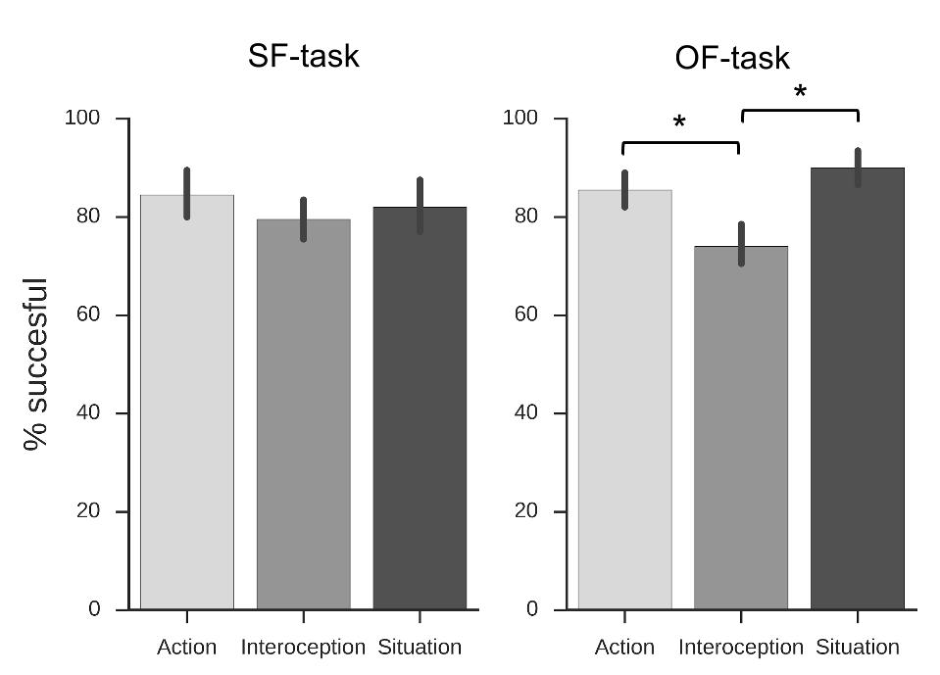
\includegraphics{_bookdown_files/shared-states-files/figures/figure_S1.pdf}
\caption{\label{fig:fig-shared-states-S1}Mean percentage of trials successfully executed for the SF-task (left panel) and OF-task (right panel). Error bars indicate 95\% confidence intervals. A one-way ANOVA of the success-rates of the SF-task (left-panel) indicated no significant overall differences, \emph{F}(2, 17) = 1.03, p = 0.38. In the OF-task (right panel) however, a one-way ANOVA indicated that success-rates differed significantly between classes, \emph{F}(2, 17) = 17.74, \emph{p} \textless{} 0.001. Follow-up pairwise comparisons (Bonferroni corrected, two tailed) revealed that interoception-trials (\emph{M} = 74.00, \emph{SE} = 2.10) were significantly less successful (\emph{p} \textless{} 0.001) than both action-trials (\emph{M} = 85.50, \emph{SE} = 1.85) and situation trials (\emph{M} = 90.00, \emph{SE} = 1.92).}
\end{figure}



\newpage
\pagestyle{empty}
\blandscape

\hypertarget{optimization-results}{%
\section{Optimization results}\label{optimization-results}}

\floatplacement{figure}{H}
\begin{figure}
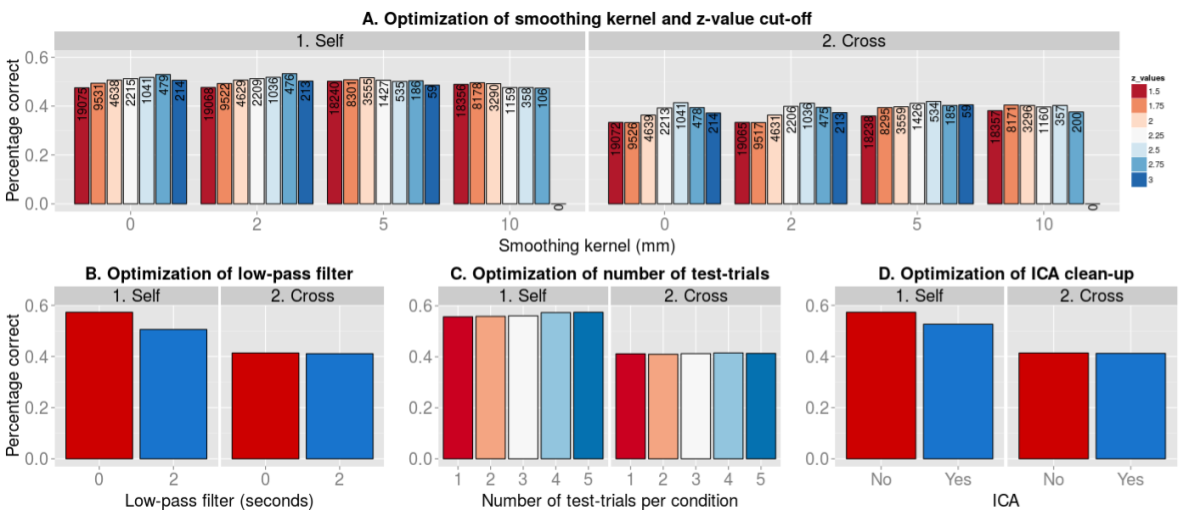
\includegraphics[width=0.9\linewidth,height=0.9\textheight]{_bookdown_files/shared-states-files/figures/figure_S2} \caption{Results of the parameter-optimization procedure. Reported scores reflect the classification scores averaged over subjects and classes (i.e.~the diagonal of the confusion matrix). All optimization analyses were iterated 5000 times. \textbf{A}) Classification results for different smoothing kernels (0, 2, 5, and 10 mm) and z-value threshold for differentiation scores during feature selection (see MVPA pipeline section in the main text for a description of the particular feature selection method we employed). Numbers reflect the average number of voxels selected across iterations. \textbf{B}) Classification results of using a low-pass filter (2 seconds) or not. \textbf{C}) Classification results for different numbers of test-trials per class (1 to 5). \textbf{D}) Classification results when preprocessing the data with Independent Component Analysis (ICA) or not.}\label{fig:fig-shared-states-S2}
\end{figure}



\elandscape
\newpage
\pagestyle{empty}

\begingroup\fontsize{10}{12}\selectfont

\begin{ThreePartTable}
\begin{TableNotes}[para]
\item \textit{Note: } 
\item The first set of parameters we evaluated in the optimization-set were different smoothing factors and feature selection thresholds (see MVPA pipeline section in the main text). On average, across the self- and cross-analysis, a 5 mm smoothing kernel yielded the best results in combination with a feature selection threshold of 2.25, which we rounded up to 2.3 as this number represents a normalized (z-transformed) score, which corresponds to the top 1\% scores within a normal distribution. Next, the difference between using a low-pass (of 2 seconds, i.e. 1 TR) versus none was assessed, establishing no low-pass filter as the optimal choice. Next, different numbers of test-trials (1 to 5) per class per iteration were assessed. Four trials yielded the best results. Lastly, the effect of “cleaning” the data with an independent component analysis was examined (FSL: MELODIC and FIX; Salimi-Khorshidi et al., 2014). Not performing ICA yielded the best results. These parameters – 5 mm smoothing kernel, 2.3 feature selection thresholded, no low-pass filter, and four test-trials per iteration – were subsequently used in the analysis of the validation set.
\end{TableNotes}
\begin{longtabu} to \linewidth {>{\raggedright}X>{\raggedright}X>{\raggedright}X}
\caption{\label{tab:tab-shared-states-S2}Parameters assessed in the optimization set}\\
\toprule
Parameter & Options & Final choice\\
\midrule
Smoothing kernel & 0 mm, 2 mm, 5 mm, 10 mm & 5 mm\\
Feature selection threshold & 1.5, 1.75, 2, 2.25, 2.5, 2.75, 3 & 2.3\\
Number of test-trials & 1, 2, 3, 4, 5 & 4\\
Low-pass filter & 2 seconds vs. none & None\\
ICA denoising & ICA vs. no ICA & No ICA\\
\bottomrule
\insertTableNotes
\end{longtabu}
\end{ThreePartTable}
\endgroup{}

\begin{figure}
\centering
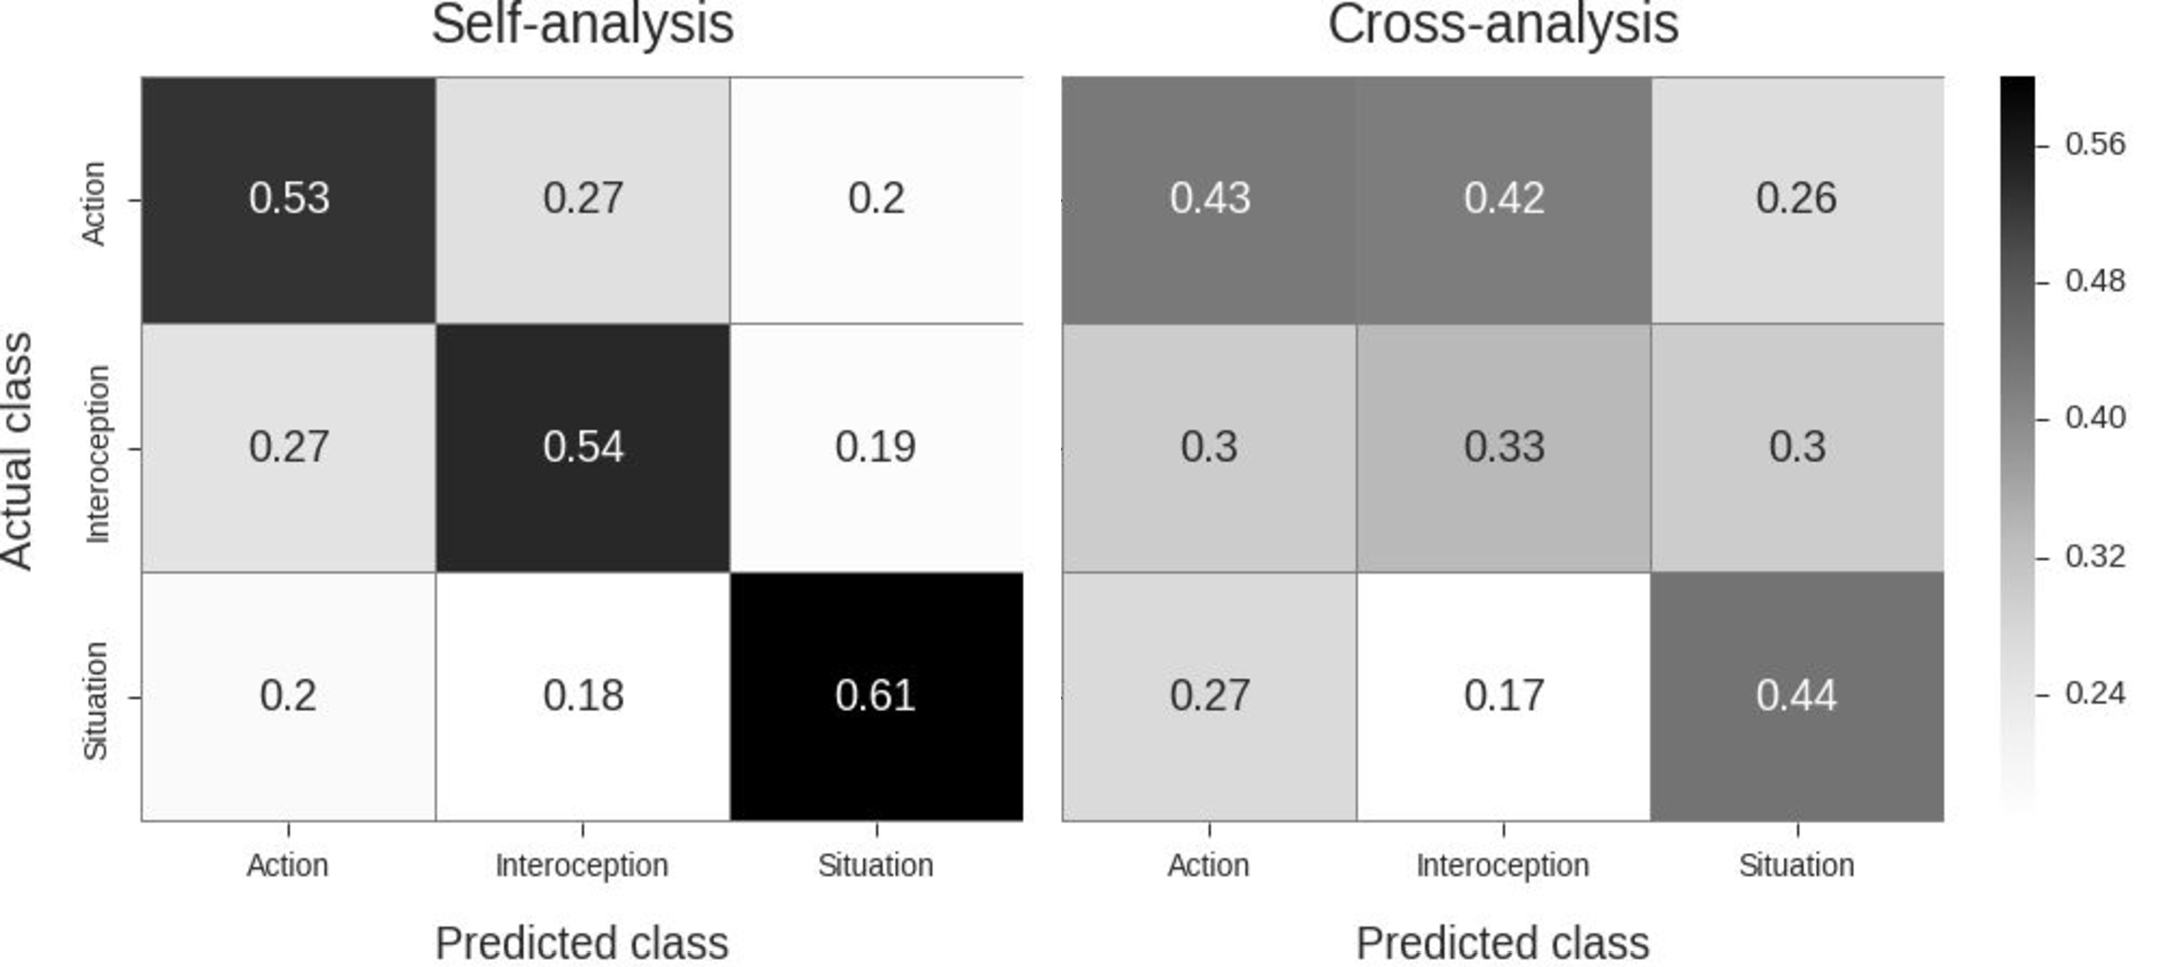
\includegraphics{_bookdown_files/shared-states-files/figures/figure_S3.pdf}
\caption{\label{fig:fig-shared-states-S3}Confusion matrices displaying precision-values yielded by the classification analysis of the optimization dataset with the final set of parameters. Because no permutation statistics were calculated for the optimization set, significance was calculated using a one-sample independent \emph{t}-test against chance-level classification (i.e.~0.333) for each cell in the diagonal of the confusion matrices. Here, all t-statistics use a degrees of freedom of 12 (i.e.~13 subjects - 1) and are evaluated against a significance level of 0.05, Bonferroni-corrected. For the diagonal of the self-analysis confusion matrix, all values were significantly above chance-level, all \emph{p} \textless{} 0.0001. For the diagonal of the cross-analysis confusion matrix, both the action (43\% correct) and situation (44\% correct) classes scored significantly above chance, \emph{p} = 0.014 and \emph{p} = 0.0007 respectively. Interoception was classified at chance level, \emph{p} = 0.99, which stands in contrast with the results in the validation-set.}
\end{figure}



\newpage
\pagestyle{empty}

\hypertarget{bagging-procedure}{%
\section{Bagging procedure}\label{bagging-procedure}}

\floatplacement{figure}{H}

\begin{figure}
\centering
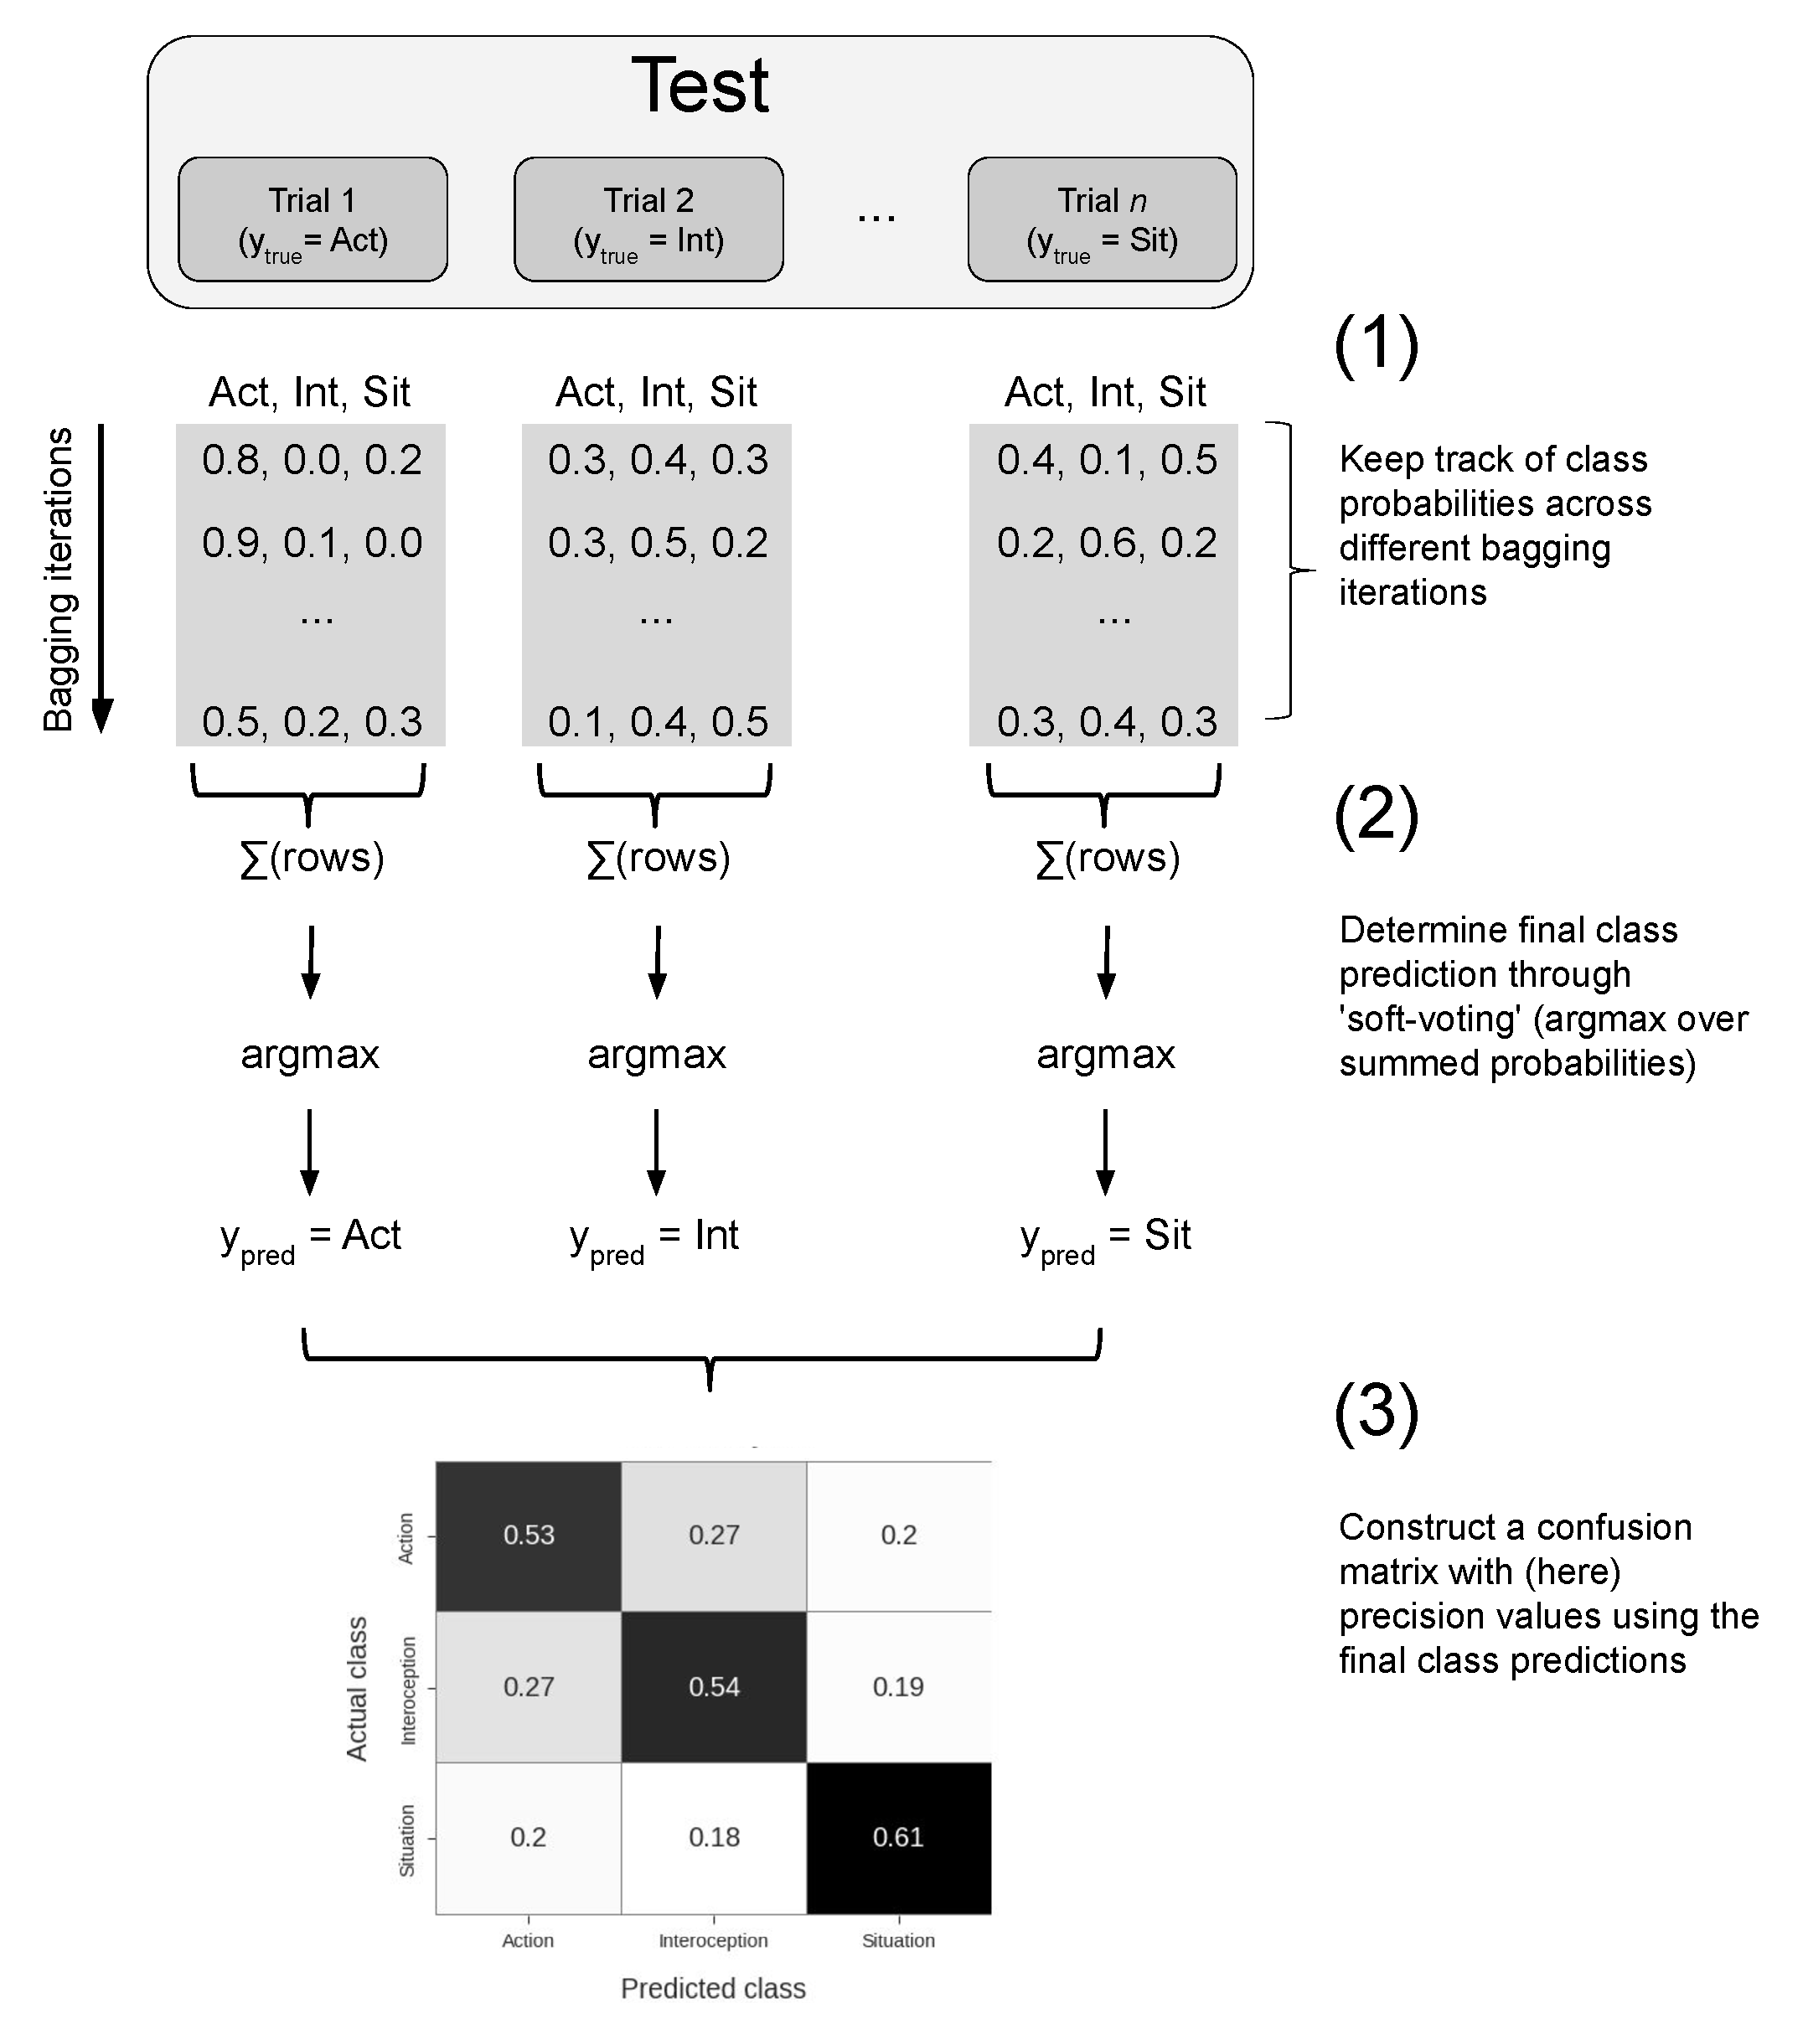
\includegraphics{_bookdown_files/shared-states-files/figures/figure_S4.pdf}
\caption{\label{fig:fig-shared-states-S4}Schematic overview of the bagging procedure. Class probabilities across different bagging iterations are summed and the class with the maximum probability determines each trial's final predicted class, which are subsequently summarized in a confusion matrix on which final recall/precision scores are calculated.}
\end{figure}



\newpage
\pagestyle{empty}

\hypertarget{precision-vs.-recall}{%
\section{Precision vs.~recall}\label{precision-vs.-recall}}

\floatplacement{figure}{H}

\begin{figure}
\centering
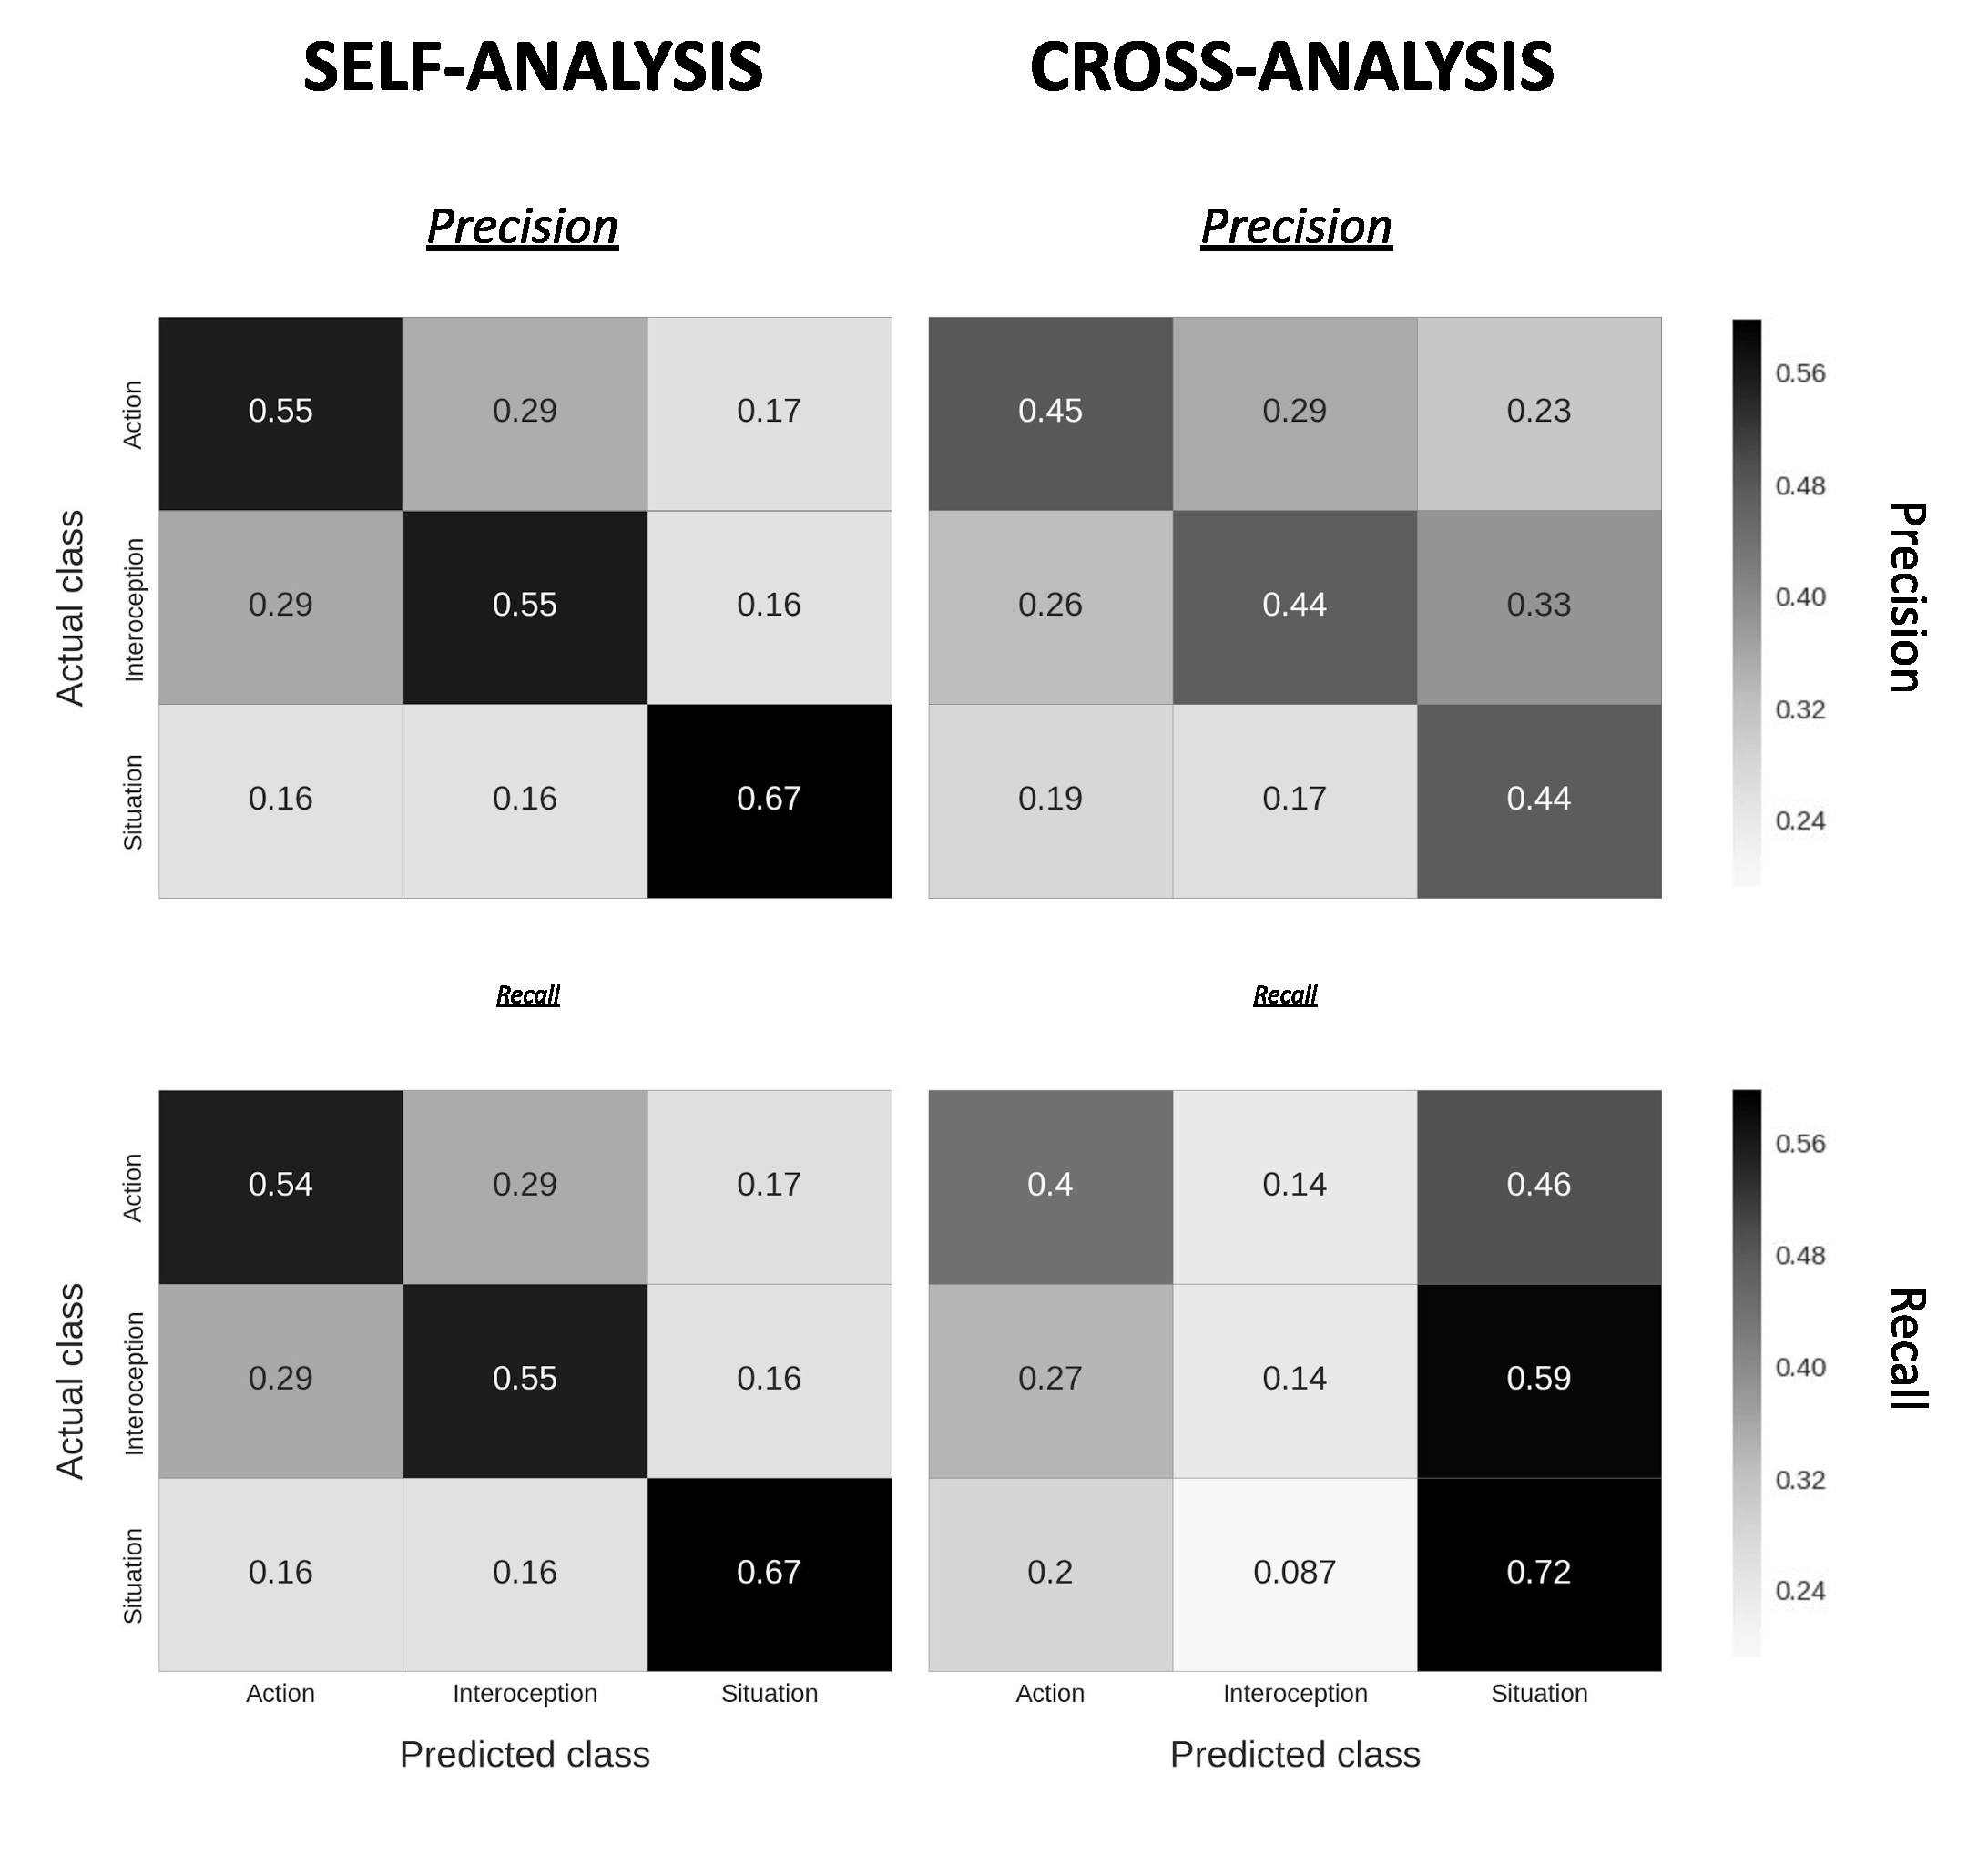
\includegraphics{_bookdown_files/shared-states-files/figures/figure_S5.pdf}
\caption{\label{fig:fig-shared-states-S5}A comparison between precision and recall confusion matrices of the self- and cross-analysis of the validation dataset. Precision refers to the amount of true positive predictions of a given class relative to all predictions for that class. Recall refers to the amount of true positive predictions of a given class relative to the total number of samples in that class. In the self-analysis, all classes were decoded significantly above chance for both precision and recall (all \emph{p} \textless{} 0.001). In the cross-analysis, all classes were decoded significantly above chance for precision (all \emph{p} \textless{} 0.001); for recall both action and situation were decoded significantly above chance (\emph{p} = 0.0013 and \emph{p} \textless{} 0.001, respectively), while interoception was decoded below chance. All \emph{p}-values were calculated using a permutation test with 1300 permutations (as described in the Methods section in the main text). When comparing precision and recall scores for both analyses, precision and recall showed very little differences in the self-analysis, while the cross-analysis shows a clear difference between metrics, especially for interoception and situation. For the interoception class, the relatively high precision score (44\%) compared to its recall score (14\%) suggests that trials are very infrequently classified as interoception, but when they are, it is (relatively) often correct. For the situation class, the relatively high recall score (72 \%) compared to its precision score (44\%) suggests that situation is strongly over-classified, which is especially clear in the lower-right confusion matrix, which indicates that 59\% of the interoception-trials are misclassified as situation-trials.}
\end{figure}



\newpage
\pagestyle{empty}

\hypertarget{self-vs.-other-classification}{%
\section{Self vs.~other classification}\label{self-vs.-other-classification}}

\floatplacement{figure}{H}

\begin{figure}
\centering
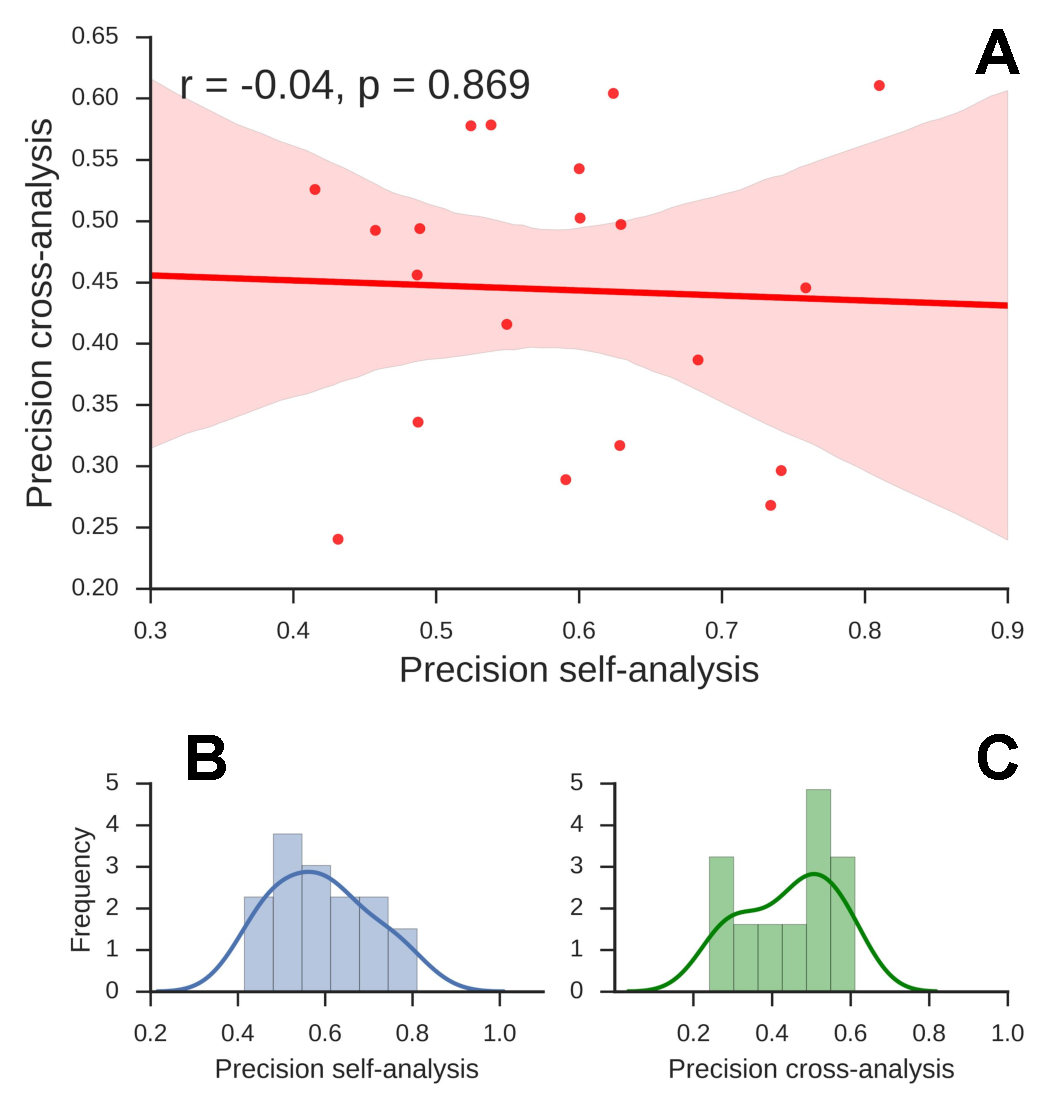
\includegraphics{_bookdown_files/shared-states-files/figures/figure_S6.pdf}
\caption{\label{fig:fig-shared-states-S6}Relation between self- and cross-analysis scores across subjects and their respective distributions. Note that the scores here represent the average of the class-specific precision scores. \textbf{A}) There is no significant correlation between precision-scores on the self-analysis and the corresponding scores on the cross-analysis, \emph{r} = -0.04, \emph{p} = .86, implying that classification scores in the self-analysis is not predictive of scores in the cross-analysis. \textbf{B}) The distribution of precision-scores in the self-analysis, appearing to be normally distributed. \textbf{C}) The distribution of precision-scores in the cross-analysis, on the other hand, appears to be bimodal, with one group of subjects having scores around chance level (0.333) while another group of subjects clearly scores above chance level (see individual scores and follow-up analyses in (ref:fig-shared-states-S4).}
\end{figure}



\newpage
\pagestyle{empty}
\floatplacement{figure}{H}

\begin{figure}
\centering
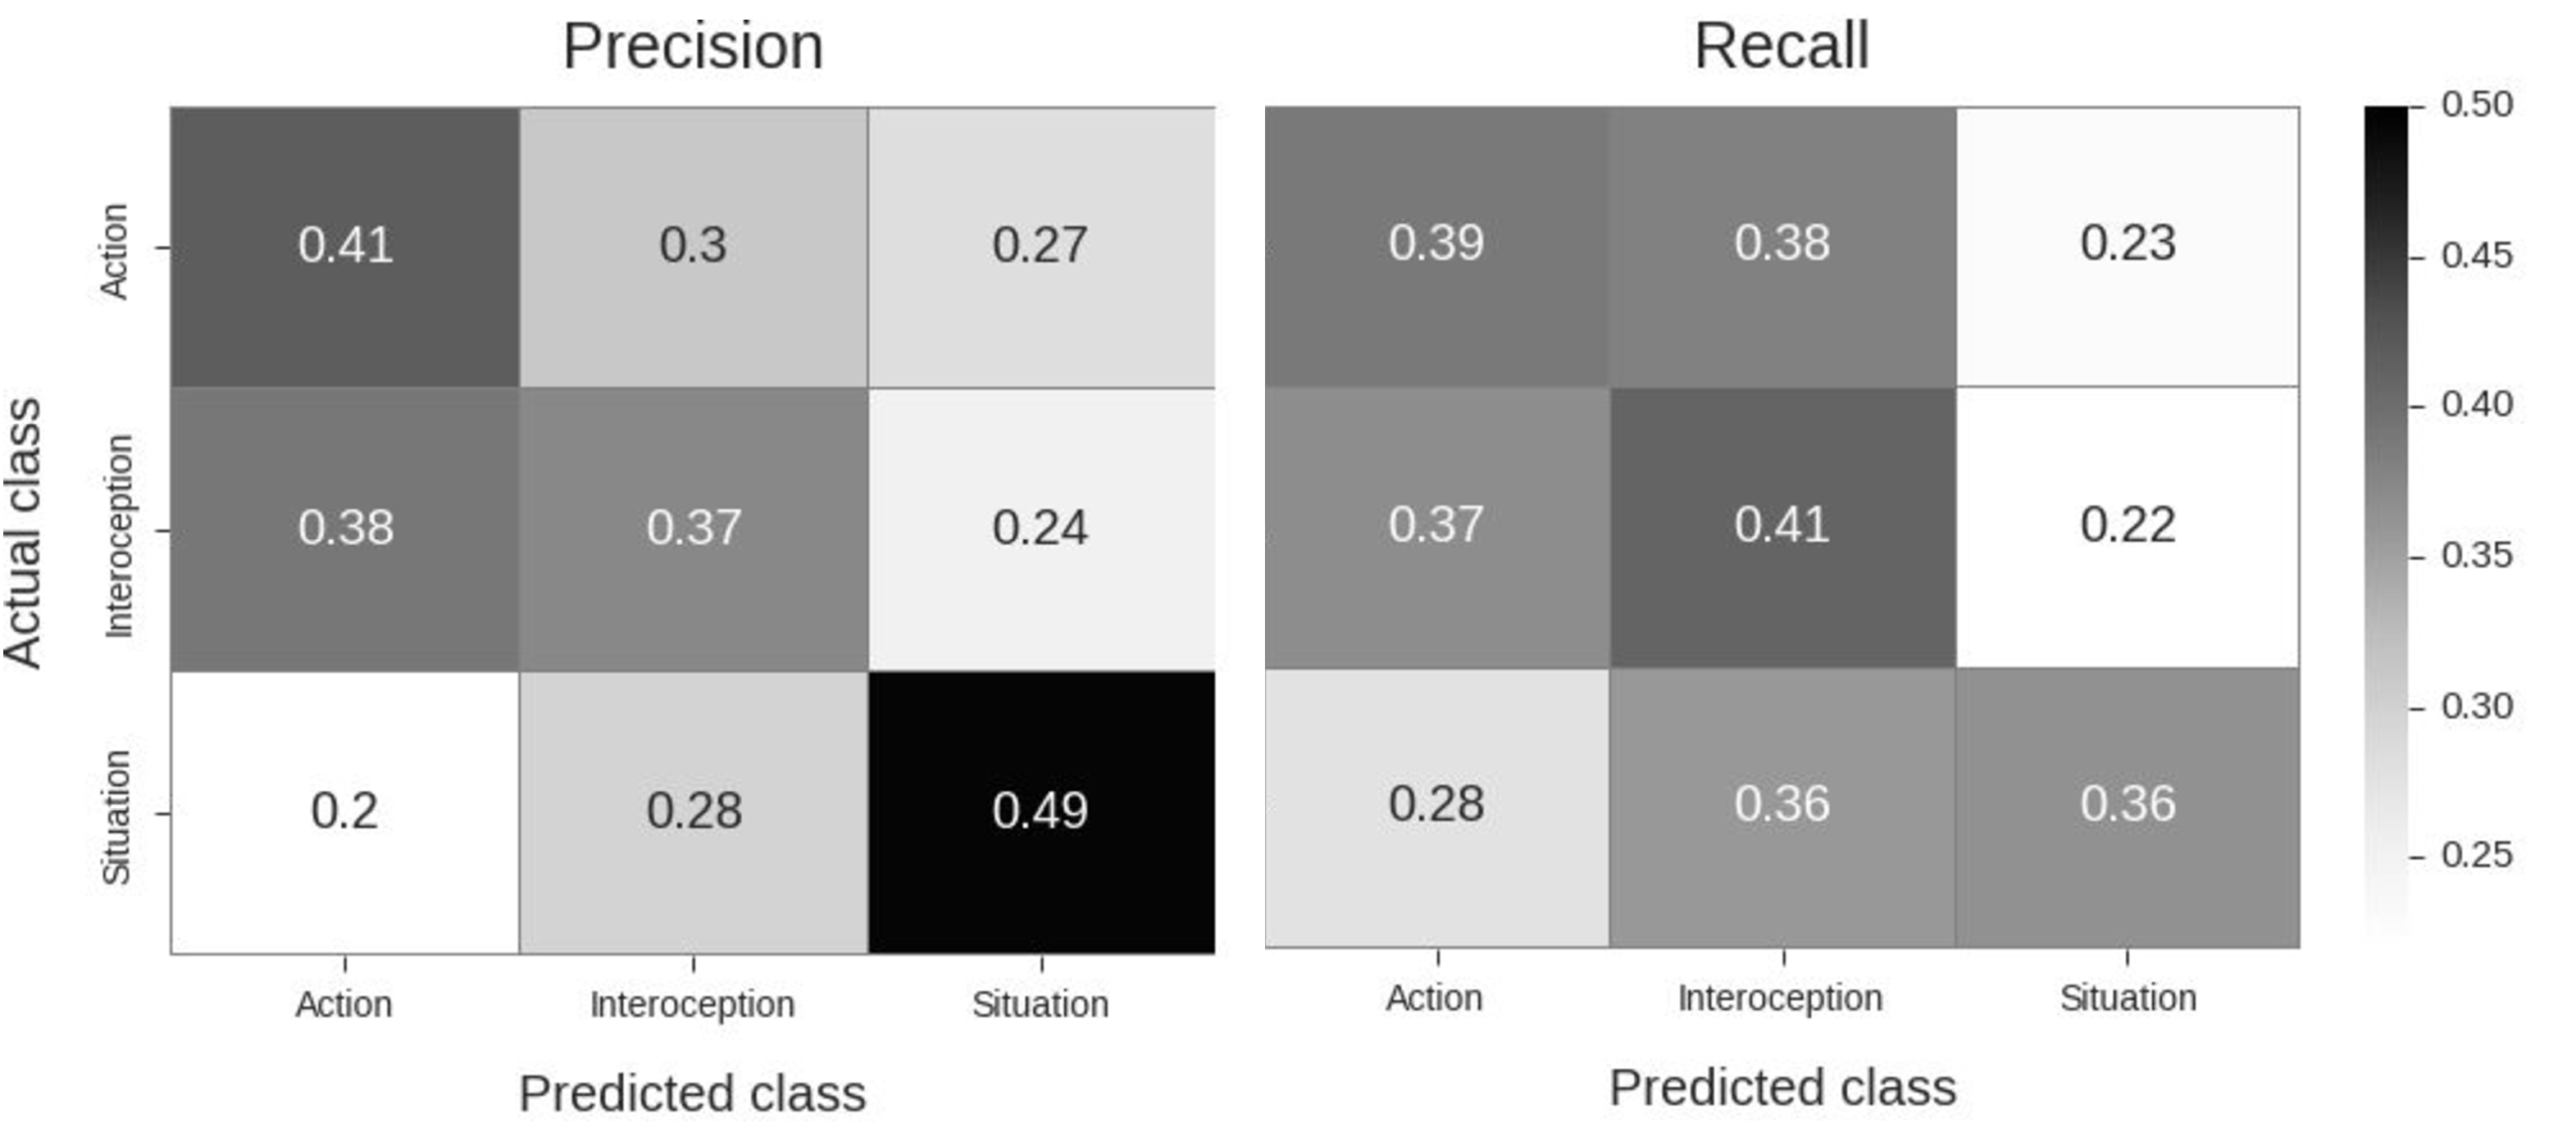
\includegraphics{_bookdown_files/shared-states-files/figures/figure_S7.pdf}
\caption{\label{fig:fig-shared-states-S7}Confusion matrices with precision (left matrix) and recall (right matrix) estimates of the other-to-self decoding analysis. The MVPA-pipeline used was exactly the same as for the (self-to-other) cross-analysis in the main text. \emph{P}-values corresponding to the classification scores were calculated using a permutation analysis with 1000 permutations of the other-to-self analysis with randomly shuffled class-labels. Similar to the self-to-other analysis, the precision-scores for all classes in the other-to-self analysis were significant, \emph{p}(action) \textless{} 0.001, \emph{p}(interoception) = 0.008, \emph{p}(situation) \textless{} 0.001. For recall, classification scores for action and interoception were significant (both \emph{p} \textless{} 0.001), but not significant for situation (\emph{p} = 0.062). The discrepancy between the self-to-other and other-to-self decoding analyses can be explained by two factors. First, the other-to-self classifier was trained on fewer samples (i.e.~90 trials) than the self-to-other classifier (which was trained on 120 trials), which may cause a substantial drop in power. Second, the preprocessing pipeline and MVPA hyperparameters were optimized based on the self-analysis and self-to-other cross-analysis. Given the vast differences between the nature of the self- and other-data, these optimal preprocessing and MVPA hyperparameters for the original analyses may not cross-validate well to the other-to-self decoding analysis.}
\end{figure}



\newpage
\pagestyle{empty}

\hypertarget{condition-average-results}{%
\section{Condition-average results}\label{condition-average-results}}

\floatplacement{figure}{H}

\begin{figure}
\centering
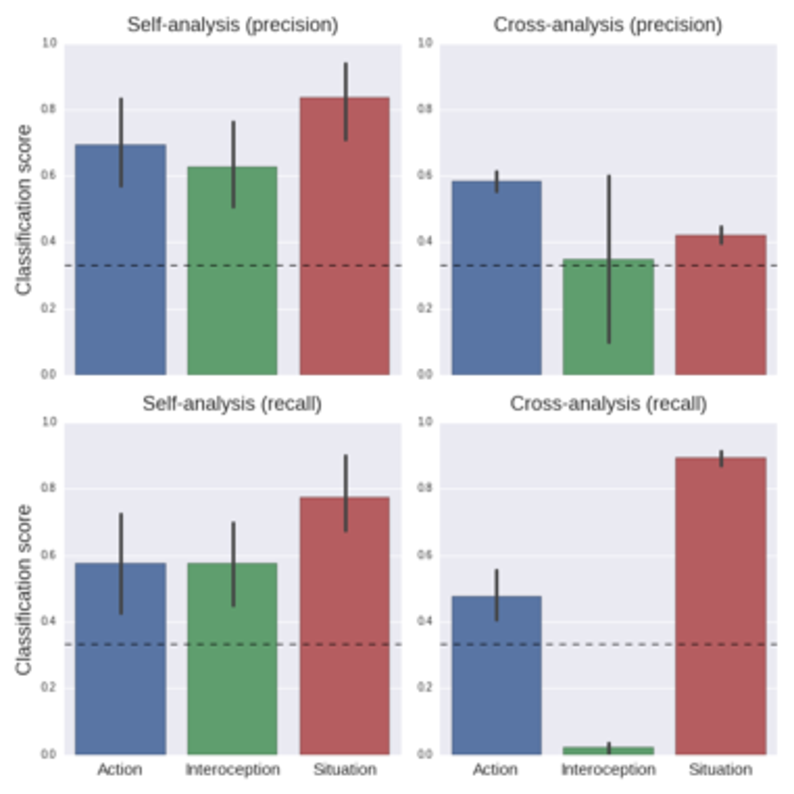
\includegraphics{_bookdown_files/shared-states-files/figures/figure_S8.pdf}
\caption{\label{fig:fig-shared-states-S8}Results of MVPA analyses using condition-average voxel patterns across subjects instead of single-trial patterns within subjects. Here, patterns are estimated in a GLM in which each condition, as opposed to each trial, is modeled with a single regressor, from which whole-brain t-value patterns were extracted. In this condition-average multi-voxel pattern analysis, condition-average patterns across subjects were used as samples. The condition-average patterns were extracted from the univariate first-level contrasts. In total, this yielded 120 samples for the self-data (3 conditions x 2 runs x 20 participants) and 60 samples for the other-data (3 conditions * 20 participants). For these analyses, the same hyperparameters were used as the original analyses reported in the main text, except with regard to the cross-validation and bagging procedure. Here, we used (stratified) 10-fold cross-validation without bagging. The upper panels show precision scores (per class) for the self- and (self-to-other) cross-analysis; the lower panels show results from the same analyses but expressed in recall-estimates (error bars indicate 95\% confidence intervals). Apart from interoception in the cross-analysis (both precision and recall), all scores were significant (p \textless{} 0.001) in a permutation test with 1000 permutations. These results largely replicate our findings as reported in the main text. This suggests that the neural patterns involved in self-focused emotional imagery and other-focused emotion understanding are relatively consistent in terms of spatial distribution across subjects. We explain this consistency by assuming that our tasks engage domain-general psychological processes that are present in all individuals.}
\end{figure}



\newpage
\pagestyle{empty}

\hypertarget{individual-subject-scores}{%
\section{Individual subject scores}\label{individual-subject-scores}}

\begingroup\fontsize{10}{12}\selectfont

\begin{ThreePartTable}
\begin{TableNotes}[para]
\item \textit{Note: } 
\item Supplementary Table 3 suggests individual variability in the extent to which neural resources are shared between self- and other-focused processes. In the SF-task all subjects demonstrated a mean classification score well above .33 (i.e., score associated with chance). When generalizing the SF-classifier to the OF-task, however, the classification scores appear to be bimodally distributed (see Supplementary Figure 5C). As can be seen in Table 3, some subjects demonstrated a relatively high mean classification score (i.e., > .45), whereas other subjects demonstrated a classification score at chance level or lower. Note that there is no significant difference between the OF classification scores for subjects who participated in the experiment for the first or second time (“Session” column in table; *t*(18) = 1.73, p = 0.10), nor for subjects who were or were not part of the optimization-set (“Part of optimization-set?” column in table; *t*(18) = -.95, p = 0.35), suggesting that inclusion in the optimization-set or session ordering is not a confound in the analyses. Regarding individual variability in self-other neural overlap, it is important to note that in the field of embodied cognition, there is increasing attention for the idea that simulation is both individually and contextually dynamic (Oosterwijk \& Barrett, 2014; Winkielman, Niedenthal, Wielgosz \& Kavanagh, 2015; see also Barrett, 2009). To better distinguish between meaningful individual variation and variation due to other factors (e.g., random noise), future research should test a priori formulated hypotheses about how and when individual variation is expected to occur. 
\end{TableNotes}
\begin{longtabu} to \linewidth {>{\raggedleft}X>{\raggedleft}X>{\raggedleft}X>{\raggedleft}X>{\raggedright}X}
\caption{\label{tab:tab-shared-states-S3}Mean general classification scores per subject for the self- and cross-analysis on the validation-set only.}\\
\toprule
Subject nr. & Self-analysis precision & Cross-analysis precision & Session & Part of optimization-set?\\
\midrule
1 & 0.758 & 0.445 & 2 & y\\
2 & 0.487 & 0.336 & 2 & y\\
3 & 0.629 & 0.316 & 1 & y\\
4 & 0.524 & 0.577 & 2 & y\\
5 & 0.457 & 0.492 & 1 & y\\
\addlinespace
6 & 0.741 & 0.296 & 2 & y\\
7 & 0.600 & 0.542 & 1 & y\\
8 & 0.431 & 0.240 & 2 & y\\
9 & 0.629 & 0.497 & 1 & y\\
10 & 0.734 & 0.268 & 2 & y\\
\addlinespace
11 & 0.683 & 0.386 & 1 & y\\
12 & 0.415 & 0.525 & 2 & y\\
13 & 0.623 & 0.604 & 1 & y\\
14 & 0.810 & 0.610 & 1 & n\\
15 & 0.538 & 0.578 & 1 & n\\
\addlinespace
16 & 0.486 & 0.455 & 1 & n\\
17 & 0.549 & 0.415 & 1 & n\\
18 & 0.488 & 0.494 & 1 & n\\
19 & 0.590 & 0.289 & 1 & n\\
20 & 0.600 & 0.502 & 1 & n\\
\bottomrule
\insertTableNotes
\end{longtabu}
\end{ThreePartTable}
\endgroup{}

\newpage
\pagestyle{empty}

\hypertarget{brain-region-importance}{%
\section{Brain region importance}\label{brain-region-importance}}

\begingroup\fontsize{10}{12}\selectfont

\begin{ThreePartTable}
\begin{TableNotes}[para]
\item \textit{Note: } 
\item Brain regions were extracted from the Harvard-Oxford (bilateral) Cortical atlas. A minimum threshold for the probabilistic masks of 20 was chosen to minimize overlap between adjacent masks while maximizing coverage of the entire brain. The column *k* represents the absolute number of above-threshold voxels in the masks. The columns *Max*, *Mean*, and *Std* represent the maximum, mean, and standard deviation from the *t*-values included in the masks. Note that the *t*-values, corresponding to the mean weight across subjects normalized by the standard error of the weights across subjects (after correcting for a positive bias when taking the absolute of the weights), were thresholded at a minimum of 1.75, referring to a *p*-value of 0.05 of a one-sided *t*-test against zero with 19 degrees of freedom (i.e. *n* – 1). Note that this *t*-value map was not corrected for multiple comparisons, and is intended to visualize which regions in the brain were generally involved in our sample of subjects. The *X*, *Y*, and *Z* columns represent the MNI152 (2mm) coordinates of the peak (i.e. max) *t*-value for each listed brain region.
\end{TableNotes}
\begin{longtabu} to \linewidth {>{\raggedright}X>{\raggedleft}X>{\raggedleft}X>{\raggedleft}X>{\raggedleft}X}
\caption{\label{tab:tab-shared-states-S4}Most important voxels in terms of their average weight across iterations and subjects.}\\
\toprule
Brain region & k & Max & Mean & Std\\
\midrule
Frontal pole & 1827 & 5.05 & 2.35 & 0.52\\
Occipital pole & 1714 & 5.15 & 2.45 & 0.56\\
Supramarginal gyrus anterior & 1573 & 7.48 & 2.84 & 0.91\\
Lateral occipital cortex superior & 1060 & 4.52 & 2.18 & 0.39\\
Lateral occipital cortex inferior & 923 & 4.73 & 2.36 & 0.49\\
\addlinespace
Angular gyrus & 856 & 4.52 & 2.24 & 0.40\\
Supramarginal gyrus posterior & 806 & 4.49 & 2.29 & 0.45\\
Middle temporal gyrus temporo-occipital & 798 & 4.00 & 2.33 & 0.48\\
Temporal pole & 711 & 4.38 & 2.37 & 0.54\\
Precentral gyrus & 568 & 3.54 & 2.14 & 0.31\\
\addlinespace
Superior temporal gyrus posterior & 549 & 3.64 & 2.27 & 0.41\\
Superior frontal gyrus & 510 & 3.83 & 2.18 & 0.38\\
Postcentral gyrus & 489 & 4.61 & 2.43 & 0.60\\
Inferior frontal gyrus parstriangularis & 488 & 4.22 & 2.35 & 0.50\\
Inferior frontal gyrus parsopercularis & 441 & 3.54 & 2.14 & 0.31\\
\addlinespace
Middle temporal gyrus posterior & 417 & 5.68 & 2.34 & 0.52\\
Occipital fusiform & 400 & 4.28 & 2.14 & 0.37\\
Middle temporal gyrus anterior & 398 & 5.68 & 2.58 & 0.76\\
Middle frontal gyrus & 300 & 3.01 & 2.06 & 0.25\\
Precuneus & 282 & 3.34 & 2.14 & 0.31\\
\bottomrule
\insertTableNotes
\end{longtabu}
\end{ThreePartTable}
\endgroup{}

\hypertarget{general-note-about-tables-with-voxel-coordinates}{%
\section{General note about tables with voxel-coordinates}\label{general-note-about-tables-with-voxel-coordinates}}

In order to keep the Supplementary materials concise and orderly, we chose not to include the actual tables with the peak coordinates of all significant clusters of the univariate analyses of the self- and other-task data (as these would amount to 25 pages). These tables, however, can be downloaded (as simple tab-separated-value files) from the study's \href{https://github.com/lukassnoek/SharedStates}{Github respository}. The voxel tables are listed under: \texttt{SharedStates/RESULTS/Voxel\_tables/*.tsv} (see green box in image below), and can be downloaded by cloning the remote Github repository locally or downloading the ZIP-file from the website (see red box in image below).

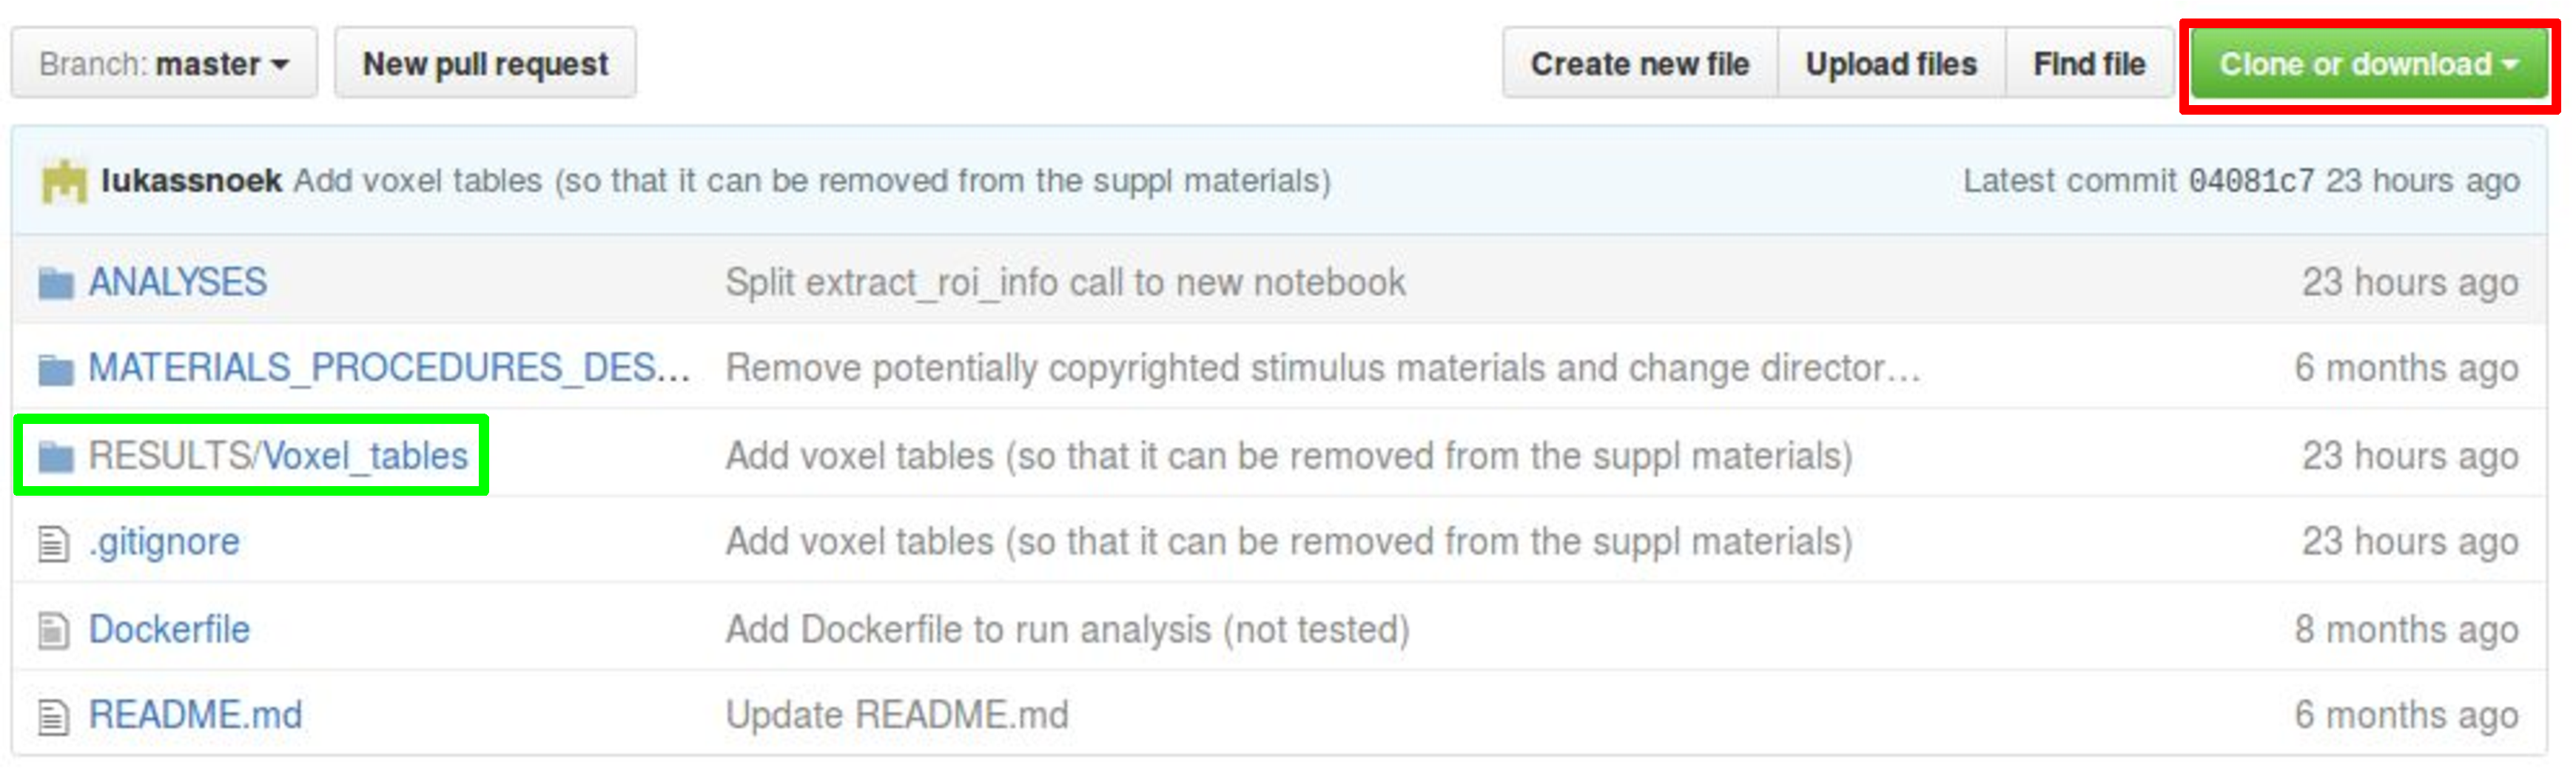
\includegraphics{_bookdown_files/shared-states-files/figures/github.pdf}

\hypertarget{confounds-decoding-supplement}{%
\chapter{Supplement to Chapter \ref{confounds-decoding}}\label{confounds-decoding-supplement}}

\hypertarget{morbid-curiosity-supplement}{%
\chapter{Supplement to Chapter \ref{morbid-curiosity}}\label{morbid-curiosity-supplement}}

\hypertarget{au-limitations-supplement}{%
\chapter{Supplement to Chapter \ref{au-limitations}}\label{au-limitations-supplement}}

\hypertarget{facial-expression-models-supplement}{%
\chapter{Supplement to Chapter \ref{facial-expression-models}}\label{facial-expression-models-supplement}}

\hypertarget{resources-supplement}{%
\chapter{Data, code and materials}\label{resources-supplement}}

\backmatter

\hypertarget{bibliography}{%
\chapter*{Bibliography}\label{bibliography}}
\addcontentsline{toc}{chapter}{Bibliography}

\markboth{\MakeUppercase{Bibliography}}{} % have to explicitly state what to put in the heading (bug in bookdown?)
%format the references so they have a hanging indent. Remove these (and the \endgroup command) if you want regular indentation.
\begingroup
\hspace{\parindent}
\setlength{\parindent}{-0.25in}
\setlength{\leftskip}{0.25in}
\setlength{\parskip}{0pt}

\hypertarget{refs}{}
\leavevmode\hypertarget{ref-anderson2016precis}{}%
Anderson, M. L. (2016). Précis of after phrenology: Neural reuse and the interactive brain. \emph{Behavioral and Brain Sciences}, \emph{39}.

\leavevmode\hypertarget{ref-andrews2014default}{}%
Andrews-Hanna, J. R., Smallwood, J., \& Spreng, R. N. (2014). The default network and self-generated thought: Component processes, dynamic control, and clinical relevance. \emph{Annals of the New York Academy of Sciences}, \emph{1316}(1), 29.

\leavevmode\hypertarget{ref-barrett2009variety}{}%
Barrett, L. F. (2009). Variety is the spice of life: A psychological construction approach to understanding variability in emotion. \emph{Cognition and Emotion}, \emph{23}(7), 1284--1306.

\leavevmode\hypertarget{ref-barrett2012emotions}{}%
Barrett, L. F. (2012). Emotions are real. \emph{Emotion}, \emph{12}(3), 413.

\leavevmode\hypertarget{ref-barrett2013large}{}%
Barrett, L. F., \& Satpute, A. B. (2013). Large-scale brain networks in affective and social neuroscience: Towards an integrative functional architecture of the brain. \emph{Current Opinion in Neurobiology}, \emph{23}(3), 361--372.

\leavevmode\hypertarget{ref-barrett2015interoceptive}{}%
Barrett, L. F., \& Simmons, W. K. (2015). Interoceptive predictions in the brain. \emph{Nature Reviews Neuroscience}, \emph{16}(7), 419--429.

\leavevmode\hypertarget{ref-barsalou2009simulation}{}%
Barsalou, L. W. (2009). Simulation, situated conceptualization, and prediction. \emph{Philosophical Transactions of the Royal Society B: Biological Sciences}, \emph{364}(1521), 1281--1289.

\leavevmode\hypertarget{ref-bastiaansen2009evidence}{}%
Bastiaansen, J. A., Thioux, M., \& Keysers, C. (2009). Evidence for mirror systems in emotions. \emph{Philosophical Transactions of the Royal Society B: Biological Sciences}, \emph{364}(1528), 2391--2404.

\leavevmode\hypertarget{ref-binder2009semantic}{}%
Binder, J. R., Desai, R. H., Graves, W. W., \& Conant, L. L. (2009). Where is the semantic system? A critical review and meta-analysis of 120 functional neuroimaging studies. \emph{Cerebral Cortex}, \emph{19}(12), 2767--2796.

\leavevmode\hypertarget{ref-breiman1996bagging}{}%
Breiman, L. (1996). Bagging predictors. \emph{Machine Learning}, \emph{24}(2), 123--140.

\leavevmode\hypertarget{ref-brosch2013implicit}{}%
Brosch, T., Bar-David, E., \& Phelps, E. A. (2013). Implicit race bias decreases the similarity of neural representations of black and white faces. \emph{Psychological Science}, \emph{24}(2), 160--166.

\leavevmode\hypertarget{ref-carr2003neural}{}%
Carr, L., Iacoboni, M., Dubeau, M.-C., Mazziotta, J. C., \& Lenzi, G. L. (2003). Neural mechanisms of empathy in humans: A relay from neural systems for imitation to limbic areas. \emph{Proceedings of the National Academy of Sciences}, \emph{100}(9), 5497--5502.

\leavevmode\hypertarget{ref-corradi2016cross}{}%
Corradi-Dell'Acqua, C., Tusche, A., Vuilleumier, P., \& Singer, T. (2016). Cross-modal representations of first-hand and vicarious pain, disgust and fairness in insular and cingulate cortex. \emph{Nature Communications}, \emph{7}(1), 1--12.

\leavevmode\hypertarget{ref-Craddock2009-kz}{}%
Craddock, R. C., Holtzheimer, P. E., 3rd, Hu, X. P., \& Mayberg, H. S. (2009). Disease state prediction from resting state functional connectivity. \emph{Magn. Reson. Med.}, \emph{62}(6), 1619--1628.

\leavevmode\hypertarget{ref-craig2009you}{}%
Craig, A. D., \& Craig, A. (2009). How do you feel--now? The anterior insula and human awareness. \emph{Nature Reviews Neuroscience}, \emph{10}(1).

\leavevmode\hypertarget{ref-Cuingnet2011-hv}{}%
Cuingnet, R., Gerardin, E., Tessieras, J., Auzias, G., Lehéricy, S., Habert, M.-O., Chupin, M., Benali, H., Colliot, O., \& Alzheimer's Disease Neuroimaging Initiative. (2011). Automatic classification of patients with alzheimer's disease from structural MRI: A comparison of ten methods using the ADNI database. \emph{Neuroimage}, \emph{56}(2), 766--781.

\leavevmode\hypertarget{ref-decety2011dissecting}{}%
Decety, J. (2011). Dissecting the neural mechanisms mediating empathy. \emph{Emotion Review}, \emph{3}(1), 92--108.

\leavevmode\hypertarget{ref-denny2012meta}{}%
Denny, B. T., Kober, H., Wager, T. D., \& Ochsner, K. N. (2012). A meta-analysis of functional neuroimaging studies of self-and other judgments reveals a spatial gradient for mentalizing in medial prefrontal cortex. \emph{Journal of Cognitive Neuroscience}, \emph{24}(8), 1742--1752.

\leavevmode\hypertarget{ref-ethofer2009decoding}{}%
Ethofer, T., Van De Ville, D., Scherer, K., \& Vuilleumier, P. (2009). Decoding of emotional information in voice-sensitive cortices. \emph{Current Biology}, \emph{19}(12), 1028--1033.

\leavevmode\hypertarget{ref-etzel2011impact}{}%
Etzel, J. A., Valchev, N., \& Keysers, C. (2011). The impact of certain methodological choices on multivariate analysis of fMRI data with support vector machines. \emph{Neuroimage}, \emph{54}(2), 1159--1167.

\leavevmode\hypertarget{ref-gallese2004unifying}{}%
Gallese, V., Keysers, C., \& Rizzolatti, G. (2004). A unifying view of the basis of social cognition. \emph{Trends in Cognitive Sciences}, \emph{8}(9), 396--403.

\leavevmode\hypertarget{ref-de2010standing}{}%
Gelder, B. de, Van den Stock, J., Meeren, H. K., Sinke, C. B., Kret, M. E., \& Tamietto, M. (2010). Standing up for the body. Recent progress in uncovering the networks involved in the perception of bodies and bodily expressions. \emph{Neuroscience \& Biobehavioral Reviews}, \emph{34}(4), 513--527.

\leavevmode\hypertarget{ref-gilbert2012evaluative}{}%
Gilbert, S. J., Swencionis, J. K., \& Amodio, D. M. (2012). Evaluative vs. Trait representation in intergroup social judgments: Distinct roles of anterior temporal lobe and prefrontal cortex. \emph{Neuropsychologia}, \emph{50}(14), 3600--3611.

\leavevmode\hypertarget{ref-guyon2002gene}{}%
Guyon, I., Weston, J., Barnhill, S., \& Vapnik, V. (2002). Gene selection for cancer classification using support vector machines. \emph{Machine Learning}, \emph{46}(1), 389--422.

\leavevmode\hypertarget{ref-Haxby2012-sd}{}%
Haxby, J. V. (2012). Multivariate pattern analysis of fMRI: The early beginnings. \emph{Neuroimage}, \emph{62}(2), 852--855.

\leavevmode\hypertarget{ref-Haxby2001-os}{}%
Haxby, J. V., Gobbini, M. I., Furey, M. L., Ishai, A., Schouten, J. L., \& Pietrini, P. (2001). Distributed and overlapping representations of faces and objects in ventral temporal cortex. \emph{Science}, \emph{293}(5539), 2425--2430.

\leavevmode\hypertarget{ref-haynes2015primer}{}%
Haynes, J.-D. (2015). A primer on pattern-based approaches to fMRI: Principles, pitfalls, and perspectives. \emph{Neuron}, \emph{87}(2), 257--270.

\leavevmode\hypertarget{ref-Hebart2017-jn}{}%
Hebart, M. N., \& Baker, C. I. (2017). Deconstructing multivariate decoding for the study of brain function. \emph{Neuroimage}.

\leavevmode\hypertarget{ref-jenkinson2012fsl}{}%
Jenkinson, M., Beckmann, C. F., Behrens, T. E., Woolrich, M. W., \& Smith, S. M. (2012). Fsl. \emph{Neuroimage}, \emph{62}(2), 782--790.

\leavevmode\hypertarget{ref-Jimura2012-lv}{}%
Jimura, K., \& Poldrack, R. A. (2012). Analyses of regional-average activation and multivoxel pattern information tell complementary stories. \emph{Neuropsychologia}, \emph{50}(4), 544--552.

\leavevmode\hypertarget{ref-kay2008identifying}{}%
Kay, K. N., Naselaris, T., Prenger, R. J., \& Gallant, J. L. (2008). Identifying natural images from human brain activity. \emph{Nature}, \emph{452}(7185), 352--355.

\leavevmode\hypertarget{ref-keysers2014dissociating}{}%
Keysers, C., \& Gazzola, V. (2014). Dissociating the ability and propensity for empathy. \emph{Trends in Cognitive Sciences}, \emph{18}(4), 163--166.

\leavevmode\hypertarget{ref-kriegeskorte2009circular}{}%
Kriegeskorte, N., Simmons, W. K., Bellgowan, P. S., \& Baker, C. I. (2009). Circular analysis in systems neuroscience: The dangers of double dipping. \emph{Nature Neuroscience}, \emph{12}(5), 535.

\leavevmode\hypertarget{ref-krishnan2016somatic}{}%
Krishnan, A., Woo, C.-W., Chang, L. J., Ruzic, L., Gu, X., López-Solà, M., Jackson, P. L., Pujol, J., Fan, J., \& Wager, T. D. (2016). Somatic and vicarious pain are represented by dissociable multivariate brain patterns. \emph{Elife}, \emph{5}, e15166.

\leavevmode\hypertarget{ref-kveraga2015if}{}%
Kveraga, K., Boshyan, J., Adams Jr, R. B., Mote, J., Betz, N., Ward, N., Hadjikhani, N., Bar, M., \& Barrett, L. F. (2015). If it bleeds, it leads: Separating threat from mere negativity. \emph{Social Cognitive and Affective Neuroscience}, \emph{10}(1), 28--35.

\leavevmode\hypertarget{ref-lamm2011meta}{}%
Lamm, C., Decety, J., \& Singer, T. (2011). Meta-analytic evidence for common and distinct neural networks associated with directly experienced pain and empathy for pain. \emph{Neuroimage}, \emph{54}(3), 2492--2502.

\leavevmode\hypertarget{ref-lamm2015role}{}%
Lamm, C., \& Majdandžić, J. (2015). The role of shared neural activations, mirror neurons, and morality in empathy--a critical comment. \emph{Neuroscience Research}, \emph{90}, 15--24.

\leavevmode\hypertarget{ref-lang2005international}{}%
Lang, P. J. (2005). International affective picture system (iaps): Affective ratings of pictures and instruction manual. \emph{Technical Report}.

\leavevmode\hypertarget{ref-lang1997international}{}%
Lang, P. J., Bradley, M. M., Cuthbert, B. N., \& others. (1997). International affective picture system (iaps): Technical manual and affective ratings. \emph{NIMH Center for the Study of Emotion and Attention}, \emph{1}, 39--58.

\leavevmode\hypertarget{ref-LaRocque2013-sh}{}%
LaRocque, J. J., Lewis-Peacock, J. A., Drysdale, A. T., Oberauer, K., \& Postle, B. R. (2013). Decoding attended information in short-term memory: An EEG study. \emph{J. Cogn. Neurosci.}, \emph{25}(1), 127--142.

\leavevmode\hypertarget{ref-legrand2009self}{}%
Legrand, D., \& Ruby, P. (2009). What is self-specific? Theoretical investigation and critical review of neuroimaging results. \emph{Psychological Review}, \emph{116}(1), 252.

\leavevmode\hypertarget{ref-lench2011discrete}{}%
Lench, H. C., Flores, S. A., \& Bench, S. W. (2011). Discrete emotions predict changes in cognition, judgment, experience, behavior, and physiology: A meta-analysis of experimental emotion elicitations. \emph{Psychological Bulletin}, \emph{137}(5), 834.

\leavevmode\hypertarget{ref-lindquist2012brain}{}%
Lindquist, K. A., Wager, T. D., Kober, H., Bliss-Moreau, E., \& Barrett, L. F. (2012). The brain basis of emotion: A meta-analytic review. \emph{The Behavioral and Brain Sciences}, \emph{35}(3), 121.

\leavevmode\hypertarget{ref-medford2010conjoint}{}%
Medford, N., \& Critchley, H. D. (2010). Conjoint activity of anterior insular and anterior cingulate cortex: Awareness and response. \emph{Brain Structure and Function}, \emph{214}(5-6), 535--549.

\leavevmode\hypertarget{ref-misaki2010comparison}{}%
Misaki, M., Kim, Y., Bandettini, P. A., \& Kriegeskorte, N. (2010). Comparison of multivariate classifiers and response normalizations for pattern-information fMRI. \emph{Neuroimage}, \emph{53}(1), 103--118.

\leavevmode\hypertarget{ref-mischkowski2016painkiller}{}%
Mischkowski, D., Crocker, J., \& Way, B. M. (2016). From painkiller to empathy killer: Acetaminophen (paracetamol) reduces empathy for pain. \emph{Social Cognitive and Affective Neuroscience}, \emph{11}(9), 1345--1353.

\leavevmode\hypertarget{ref-mumford2014impact}{}%
Mumford, J. A., Davis, T., \& Poldrack, R. A. (2014). The impact of study design on pattern estimation for single-trial multivariate pattern analysis. \emph{Neuroimage}, \emph{103}, 130--138.

\leavevmode\hypertarget{ref-nichols2002nonparametric}{}%
Nichols, T. E., \& Holmes, A. P. (2002). Nonparametric permutation tests for functional neuroimaging: A primer with examples. \emph{Human Brain Mapping}, \emph{15}(1), 1--25.

\leavevmode\hypertarget{ref-norman2006beyond}{}%
Norman, K. A., Polyn, S. M., Detre, G. J., \& Haxby, J. V. (2006a). Beyond mind-reading: Multi-voxel pattern analysis of fMRI data. \emph{Trends in Cognitive Sciences}, \emph{10}(9), 424--430.

\leavevmode\hypertarget{ref-Norman2006-bt}{}%
Norman, K. A., Polyn, S. M., Detre, G. J., \& Haxby, J. V. (2006b). Beyond mind-reading: Multi-voxel pattern analysis of fMRI data. \emph{Trends Cogn. Sci.}, \emph{10}(9), 424--430.

\leavevmode\hypertarget{ref-oosterwijk2014embodiment}{}%
Oosterwijk, S., \& Barrett, L. F. (2014). Embodiment in the construction of emotion experience and emotion understanding. \emph{Routledge Handbook of Embodied Cognition. New York: Routledge}, 250--260.

\leavevmode\hypertarget{ref-oosterwijk2012states}{}%
Oosterwijk, S., Lindquist, K. A., Anderson, E., Dautoff, R., Moriguchi, Y., \& Barrett, L. F. (2012). States of mind: Emotions, body feelings, and thoughts share distributed neural networks. \emph{NeuroImage}, \emph{62}(3), 2110--2128.

\leavevmode\hypertarget{ref-oosterwijk2015concepts}{}%
Oosterwijk, S., Mackey, S., Wilson-Mendenhall, C., Winkielman, P., \& Paulus, M. P. (2015). Concepts in context: Processing mental state concepts with internal or external focus involves different neural systems. \emph{Social Neuroscience}, \emph{10}(3), 294--307.

\leavevmode\hypertarget{ref-parkinson2014common}{}%
Parkinson, C., Liu, S., \& Wheatley, T. (2014). A common cortical metric for spatial, temporal, and social distance. \emph{Journal of Neuroscience}, \emph{34}(5), 1979--1987.

\leavevmode\hypertarget{ref-pedregosa2011scikit}{}%
Pedregosa, F., Varoquaux, G., Gramfort, A., Michel, V., Thirion, B., Grisel, O., Blondel, M., Prettenhofer, P., Weiss, R., Dubourg, V., \& others. (2011). Scikit-learn: Machine learning in python. \emph{The Journal of Machine Learning Research}, \emph{12}, 2825--2830.

\leavevmode\hypertarget{ref-peelen2010supramodal}{}%
Peelen, M. V., Atkinson, A. P., \& Vuilleumier, P. (2010). Supramodal representations of perceived emotions in the human brain. \emph{Journal of Neuroscience}, \emph{30}(30), 10127--10134.

\leavevmode\hypertarget{ref-pulvermuller2010active}{}%
Pulvermüller, F., \& Fadiga, L. (2010). Active perception: Sensorimotor circuits as a cortical basis for language. \emph{Nature Reviews Neuroscience}, \emph{11}(5), 351--360.

\leavevmode\hypertarget{ref-rutgen2015placebo}{}%
Rütgen, M., Seidel, E.-M., Silani, G., Riečansky, I., Hummer, A., Windischberger, C., Petrovic, P., \& Lamm, C. (2015). Placebo analgesia and its opioidergic regulation suggest that empathy for pain is grounded in self pain. \emph{Proceedings of the National Academy of Sciences}, \emph{112}(41), E5638--E5646.

\leavevmode\hypertarget{ref-sabatinelli2011emotional}{}%
Sabatinelli, D., Fortune, E. E., Li, Q., Siddiqui, A., Krafft, C., Oliver, W. T., Beck, S., \& Jeffries, J. (2011). Emotional perception: Meta-analyses of face and natural scene processing. \emph{Neuroimage}, \emph{54}(3), 2524--2533.

\leavevmode\hypertarget{ref-salimi2014automatic}{}%
Salimi-Khorshidi, G., Douaud, G., Beckmann, C. F., Glasser, M. F., Griffanti, L., \& Smith, S. M. (2014). Automatic denoising of functional mri data: Combining independent component analysis and hierarchical fusion of classifiers. \emph{Neuroimage}, \emph{90}, 449--468.

\leavevmode\hypertarget{ref-singer2012past}{}%
Singer, T. (2012). The past, present and future of social neuroscience: A european perspective. \emph{Neuroimage}, \emph{61}(2), 437--449.

\leavevmode\hypertarget{ref-spreng2009common}{}%
Spreng, R. N., Mar, R. A., \& Kim, A. S. (2009). The common neural basis of autobiographical memory, prospection, navigation, theory of mind, and the default mode: A quantitative meta-analysis. \emph{Journal of Cognitive Neuroscience}, \emph{21}(3), 489--510.

\leavevmode\hypertarget{ref-spunt2012integrative}{}%
Spunt, R. P., \& Lieberman, M. D. (2012). An integrative model of the neural systems supporting the comprehension of observed emotional behavior. \emph{Neuroimage}, \emph{59}(3), 3050--3059.

\leavevmode\hypertarget{ref-stelzer2014prioritizing}{}%
Stelzer, J., Buschmann, T., Lohmann, G., Margulies, D. S., Trampel, R., \& Turner, R. (2014). Prioritizing spatial accuracy in high-resolution fMRI data using multivariate feature weight mapping. \emph{Frontiers in Neuroscience}, \emph{8}, 66.

\leavevmode\hypertarget{ref-uddin2007self}{}%
Uddin, L. Q., Iacoboni, M., Lange, C., \& Keenan, J. P. (2007). The self and social cognition: The role of cortical midline structures and mirror neurons. \emph{Trends in Cognitive Sciences}, \emph{11}(4), 153--157.

\leavevmode\hypertarget{ref-van2009understanding}{}%
Van Overwalle, F., \& Baetens, K. (2009). Understanding others' actions and goals by mirror and mentalizing systems: A meta-analysis. \emph{Neuroimage}, \emph{48}(3), 564--584.

\leavevmode\hypertarget{ref-varoquaux2018cross}{}%
Varoquaux, G. (2018). Cross-validation failure: Small sample sizes lead to large error bars. \emph{Neuroimage}, \emph{180}, 68--77.

\leavevmode\hypertarget{ref-waytz2011two}{}%
Waytz, A., \& Mitchell, J. P. (2011). Two mechanisms for simulating other minds: Dissociations between mirroring and self-projection. \emph{Current Directions in Psychological Science}, \emph{20}(3), 197--200.

\leavevmode\hypertarget{ref-wilson2011grounding}{}%
Wilson-Mendenhall, C. D., Barrett, L. F., Simmons, W. K., \& Barsalou, L. W. (2011). Grounding emotion in situated conceptualization. \emph{Neuropsychologia}, \emph{49}(5), 1105--1127.

\leavevmode\hypertarget{ref-winkielman2015embodiment}{}%
Winkielman, P., Niedenthal, P., Wielgosz, J., Eelen, J., \& Kavanagh, L. C. (2015). \emph{Embodiment of cognition and emotion.}

\leavevmode\hypertarget{ref-wurm2015decoding}{}%
Wurm, M. F., \& Lingnau, A. (2015). Decoding actions at different levels of abstraction. \emph{Journal of Neuroscience}, \emph{35}(20), 7727--7735.

\leavevmode\hypertarget{ref-zaki2012neuroscience}{}%
Zaki, J., \& Ochsner, K. N. (2012). The neuroscience of empathy: Progress, pitfalls and promise. \emph{Nature Neuroscience}, \emph{15}(5), 675--680.

\leavevmode\hypertarget{ref-zaki2016anatomy}{}%
Zaki, J., Wager, T. D., Singer, T., Keysers, C., \& Gazzola, V. (2016). The anatomy of suffering: Understanding the relationship between nociceptive and empathic pain. \emph{Trends in Cognitive Sciences}, \emph{20}(4), 249--259.

\endgroup

\hypertarget{contributions-to-the-chapters}{%
\chapter*{Contributions to the chapters}\label{contributions-to-the-chapters}}
\addcontentsline{toc}{chapter}{Contributions to the chapters}

\chaptermark{Contributions to chapters}
\setlength{\parindent}{0pt}
\small

\hypertarget{list-of-other-publications}{%
\chapter*{List of other publications}\label{list-of-other-publications}}
\addcontentsline{toc}{chapter}{List of other publications}

\chaptermark{List of other publications}

van der Maas, H.L.J., \textbf{Snoek, L.}, \& Stevenson, C. (2021). How much intelligence is there in artificial intelligence? A 2020 update.\newline

Hoogeveen, S., \textbf{Snoek, L.}, \& Van Elk, M. (2020). Religious belief and cognitive conflict sensitivity: A preregistered fMRI study. \emph{Cortex, 129}, 247--265.\newline

van Elk, M., \& \textbf{Snoek, L.} (2020). The relationship between individual differences in gray matter volume and religiosity and mystical experiences: A preregistered voxel‐based morphometry study. \emph{European Journal of Neuroscience, 51}(3), 850--865.\newline

Van Mourik, T., \textbf{Snoek, L.}, Knapen, T., \& Norris, D. G. (2018). Porcupine: a visual pipeline tool for neuroimaging analysis. \emph{PLoS computational biology, 14}(5), e1006064.\newline

\normalsize
\setlength{\parindent}{1.5em}

\hypertarget{nederlandse-samenvatting-summary-in-dutch}{%
\chapter*{Nederlandse samenvatting (Summary in Dutch)}\label{nederlandse-samenvatting-summary-in-dutch}}
\addcontentsline{toc}{chapter}{Nederlandse samenvatting (Summary in Dutch)}

\chaptermark{Summary in Dutch}

\begin{dutch}

\emph{Replace this with the Dutch title of your thesis}

\bigskip

The summary goes here.

\end{dutch}

\hypertarget{acknowledgments}{%
\chapter*{Acknowledgments}\label{acknowledgments}}
\addcontentsline{toc}{chapter}{Acknowledgments}

\chaptermark{Acknowledgments}

This section is optional, but theses typically include acknowledgments (\textdutch{\emph{dankwoord}} in Dutch) at the end. You may want to mix languages to thank people in their native tongue (though most Dutch speakers write it entirely in Dutch). But the standard language of the thesis template is English. You can switch temporarily by wrapping the text in language tags like so: \texttt{{[}Your\ Dutch\ text\ here{]}\{lang=nl\}}. This is important for things like hyphenation to work properly.

\backmatter


\end{document}
